\documentclass[]{ccs-thesis}
% options:
% [germanthesis] - Thesis is written in German
% [plainunnumbered] - Don't print numbers on plain pages
% [earlydraft] - Settings for quick draft printouts
% [watermark] - Print current time/date at bottom of each page
% [phdthesis] - switch to PhD thesis style
% [twoside] - double sided
% [cutmargins] - text body fills complete page

% Required package
\usepackage{tikz}
\usepackage{outlines}
\usepackage[underline=true,rounded corners=false]{pgf-umlsd}
% Protocol Header file
\usepackage{bytefield}
\usepackage{makecell}
\usepackage{tabularx}
\usepackage{tabularray}
% table coloring
\usepackage{colortbl}
\usepackage{lipsum}
% block diagram
\usepackage{amsmath}
\usetikzlibrary{shapes.geometric,positioning}
% listings without linebreak
\usepackage{adjustbox}


\lstdefinestyle{customc}{
  belowcaptionskip=1\baselineskip,
  breaklines=true,
  frame=single,
  xleftmargin=\parindent,
  language=C++,
  showstringspaces=false,
  basicstyle=\footnotesize\ttfamily,
  keywordstyle=\bfseries\color{green!40!black},
  commentstyle=\itshape\color{purple!40!black},
  identifierstyle=\color{blue},
  stringstyle=\color{orange},
}

\lstset{escapechar=@,style=customc}

% Choose one of the following lines.
%\group{Cooperative Mobile Systems}
\group{Distributed Embedded Systems}

% Author name. Separate multiple authors with commas.
\author{Maximilian W. Gotthardt}
\birthday{13. July 1993}
\birthplace{Berlin}

% Title of your thesis.
\title{Evaluation of protocols \\for control stage lighting}

% Degree program.
\thesistype{Bachelor Thesis in Computer Engineering}\thesiscite{Bachelor Thesis~(Bachelorarbeit)}

% List of advisors, separated by commas. Delete if identical to referees or inapplicable.
\advisors{Anatolij Zubow}

% List of referees, separated by commas.
\referees{Falko Dressler, Thomas Sikora}

% Abbreviations own
\acrodef{RR}{Rapid Repetition}
\acrodef{MCU}{Microcontroller Unit}

% Abbreviations light protocols
\acrodef{DMX}{Digital Multiplex}
\acrodef{CANhashing}[CAN]{Content Addressable Network}{extra={when referring to the distributed hash table}}
\acrodef{CANproto}[CAN]{Controller Area Network}{extra={when referring to the bus protocol}}

% Abbreviations Networking
\acrodef{IEEE}{Institut of Electrical and Electronics Engineers}
\acrodef{OSI}{Open Systems Interconnection}
\acrodef{MSDU}{MAC Service Data Unit}
\acrodef{DL}{Data Link Layer}
\acrodef{LLC}{Locig Link Control}
\acrodef{MAC}{Media Access Control}
\acrodef{IP}{Internet Protocol}
\acrodef{CD}{Collision Detection}
\acrodef{CSMA/CA}{Carrier-sense Multiple Access with Collision Avoidance}
\acrodef{DCF}{Distributed Coordination Function}
\acrodef{PCF}{Point Coordination Function}
\acrodef{DIFS}{DCF Inter Frame Spaces}
\acrodef{SIFS}{Short Inter Frame Spaces}
\acrodef{NAV}{Network Allocation Vector}
\acrodef{PHY}{Physical Network Layer}
\acrodef{CW}{Contention Window}
\acrodef{MPDU}{Mac Protocol Data Unit}
\acrodef{DSSS}{Direct Sequence Spread Spectrum}
\acrodef{FHSS}{Frequency Hopping Spread Spectrum}
\acrodef{STA}{Station}
\acrodef{AP}{Access Point}
\acrodef{WES}{Wireless Endsystem}
\acrodef{BSS}{Basic Service Set}
\acrodef{OFDM}{Orthogonal Frequency Division Multiplexing)}
\acrodef{MIMO}{Multiple Input-Multiple Output)}
\acrodef{WLAN}{Wireless Local Area Network}
\acrodef{LAN}{Local Area Network}
\acrodef{BSSID}{Basic Service Set Identifier}
\acrodef{UDP}{User Datagram Protocol}

% Abbreviations other
\acrodef{UART}{Universal Asynchronous Receiver Transmitter}

\begin{document}

\pagenumbering{roman}

\maketitle

\thispagestyle{empty}

\cleardoublepage

\chapter*{Abstract}
\addcontentsline{toc}{chapter}{Abstract}
\begin{otherlanguage*}{american}

% about 1/2 page:
% \begin{enumerate}
% 	\item Motivation (Why do I care?)
% 	\item Problem statement (What problem are I trying to solve?)
% 	\item Approach (How did I go about it)
% 	\item Results (What's the answer?)
% 	\item Conclusion (What are the implications of the answer?)
% \end{enumerate}

In the field of lighting and stage technology, the challenge of controlling the individual installations, quickly and without complications is a recurring one. 
Established solutions are realized via cables using DMX-512a. 
However, due to the progress in radio technology, wireless solutions based on 801.11 are becoming more and more common. 

But it is a challenge to send control signals, to many individual stations and to update them multiple times a second.
Additionally a low latency and, of course, a certain reliability must be guaranteed.
This is challenged because at typical locations, such as a concert, there are often very busy frequency bands.
This thesis therefore examines an approach that attempts to reduce a large part of the overhead,
by having the stations communicate with each other on an Ad-Hoc network at the data link layer,
in order to improve the throughput.
Different approaches with broadcast and unicast are evaluated analytically and experimentally.

It can be shown that the overhead has a great influence on the transmission and that it is particularly extreme,
because so many individual stations are often only controlled with very short control signals.
The results show that the gain in throughput means that packets can be sent redundantly,
which also leads to improvements in reliability.
	
\end{otherlanguage*}

\chapter*{Kurzfassung}
\addcontentsline{toc}{chapter}{Kurzfassung}
\begin{otherlanguage*}{ngerman}
\begin{itemize}
	\item kabellose lösungen werden interessant
	\item chips werden günstiger
	\item für kleine projekte leider sehr teuere Hardware
	\item 802.11 wird als standard benutzt
	\item protokolle wie art-net könnten optimiert werden
	\item esp plattform bietet interssante möglichkeiten, wegen der geringen kosten der chips und esp-now
	\item entwicklung einer plattform die esp-now nutzt
	\item verschiedene ansätze studiert, wie broadcast und unicasts
	\item mit jeweils unterschiedlichen modifikationen
\end{itemize}

In the field of lighting and stage technology, the challenge of controlling the
individual lights, called 'fixtures', quickly and without complications is a
recurring one. 
Established solutions are realized via cables, which are difficult to install and inflexible.




Kabellose Lösungen werden durch bessere Technik und stetige Weiterentwicklung immer interessanter.
jedoch stellt es sie nach wie vor eine Herausforderung zu sein die Steuersignale des Lichtpults kabellos zu verteilen. 
denn es bekommen viele einzelne Stationen kurze Steuersignale, die ständig aktualisiert werden.



\todo{TOLJA: Wirklich noch einmal auf deutsch?}

\end{otherlanguage*}
\acresetall

\cleardoublepage
\tableofcontents
\TODO{The table of contents should fit on one page. When in doubt, adjust the \texttt{tocdepth} counter.}

\cleardoublepage
\pagenumbering{arabic}


\chapter{Introduction}
%\chapter{Einleitung}

\begin{itemize}
	\item general motivation for your work, context and goals.
	\item context: make sure to link where your work fits in
	\item problem: gap in knowledge, too expensive, too slow, a deficiency, superseded technology
	\item strategy: the way you will address the problem
	\item recommended length: 1-2 pages.
\end{itemize}

In the subject area 

====

In the field of lighting and stage technology, the challenge of controlling the individual installations, called 'fixtures', quickly and without complications is a recurring one. 
Established solutions are realized via cables.

\section{Motivation/Requirements}
\begin{itemize}
	\item Reliability
	\item .. and why 100\% Reliability is not important (pyrotechnics)
	\item Lower latency
	\item Synchronisation
	\item higher update frequency
	\item Range
\end{itemize}

\section{Challenges}
\begin{itemize}
\item low cost
\item (ESP Platform)
\item DIY community
\end{itemize}

\section{Problemstatement and Contribution WICHTIG}
\begin{itemize}
\item open source available on github [link]
\item thought-provoking impulse for different approaches
\item Protocol auf DL Layer/App Layer Ebene
\item Art-Net baseline
\item simulativ und experimentel untersucht
\end{itemize}

\section{Thesis Outline}
\begin{itemize}
	\item A First Implementation and Evaluation of the IEEE 802.11aa Group Addressed Transmission Service    
		\subitem unsosliced Repetition
		\subitem blockack
	\item Evaluation of Error Control Mechanisms for 802.11b Multicast Transmissions
		\subitem packet loss rate
		\subitem ARQ, FEC
	\item ESP-NOW communication protocol with ESP32
		\subitem ESP-NOW details
	\item The Working Principles of ESP32 and Analytical Comparision of using Low-Cost Microcontroller Modules in Embedded Systems Design
		\subitem why the ESP32 is superior over arduino
	\item Adaptive Cross-Layer Protection Strategies for Robust Scqalable Video Transmissions Over 802.11 WLANs
	\item Voice Capacity of IEEE 802.11b, 802.11a and 802.11g Wireless LANs
\end{itemize}

  
\chapter{Related Work}
% \begin{itemize}
% 	\item Wie der und der in Paper so gezeigt hat 
% 	\item Auch Ding et al haben versucht
% 	\item ...
% 	\item 10 Paper
% 	\item halbe seite
% \end{itemize}


% \begin{itemize}
% 	\item A First Implementation and Evaluation of the IEEE 802.11aa Group Addressed Transmission Service    
% 		\subitem unsosliced Repetition
% 		\subitem blockack
% 	\item Evaluation of Error Control Mechanisms for 802.11b Multicast Transmissions
% 		\subitem packet loss rate
% 		\subitem ARQ, FEC
% 	\item ESP-NOW communication protocol with ESP32
% 		\subitem ESP-NOW details
% 	\item The Working Principles of ESP32 and Analytical Comparision of using Low-Cost Microcontroller Modules in Embedded Systems Design
% 		\subitem why the ESP32 is superior over arduino
% 	\item Adaptive Cross-Layer Protection Strategies for Robust Scqalable Video Transmissions Over 802.11 WLANs
% 	\item Voice Capacity of IEEE 802.11b, 802.11a and 802.11g Wireless LANs
% \end{itemize}

The trend towards wireless solutions in all areas also affects stage technology.
However, wireless solutions often have lower throughput, latency and reliability than their wired counterparts.

Cost-effective solutions work with the 802.11 protocol, which is widely used. 
H. Kareem and D. Dunaev \cite{TheWorkingPrincipalsOfESP32} observed that
\emph{the recently growing demand for the control and automation of a wide variety of devices and gadgets has
led to a rapid expansion in embedded systems market}.
When selecting the platform for the experiments in this thesis, the ESP32 was chosen, 
which was compared analytically along with Arduino embedded systems from the two,
with the result, \emph{to highlight the advantages of the ESP32 in designing embedded systems compared to similar boards}.

Due to the fact that many individual stations are controlled in stage lighting, 
often with very short signals, this can sometimes lead to an extreme overhead.
\emph{Overhead is} 
according to Y. Xiao \cite{PerformanceEnhancement}
\emph{one of the fundamental problems of MAC inefficiency, and it includes MAC header, frame check sequence, and physical header.}
But also interframe spaces can be classified as overhead.

The impact of transmission overhead is also researched by Nurul Sarkar \cite{TheImpactOfOverheads}
he pointed out the DCF inefficiency and developed a protocol that
\emph{is a simple packet scheduling mechanism that can be used to reduce transmission overheads of DCF and to improve the performance. 
The key idea is to create a temporary buffer unit at the MAC layer for each active connection on the network 
where multiple packets are accumulated and combined into a single large packet}.
In this thesis broadcasts are used to address multiple stations 
in order to reduce overhead compared to multiple unicast transmissions.
Nurul Sarkar \cite{TheImpactOfOverheads} also took a look into 
\emph{its impact on throughput for a single-user wireless ad hoc network},
which were used in this thesis.

Addressing to multiple stations is often realized with multicasts, 
because, unlike broadcasts, acknowledgements can be sent. One approach to this is presented by Pablo Salvador et. al. 
\cite{AFirstImplementation}
they experimentally investigate the IEEE 802.11aa GATS and test block acknowledgements.
Also unsolicited retries where researched by them: 
\emph{the idea is to improve reliability with a very somple scheme, wich does not requre a 
closed loop between the sender and the receivers(s), and therefore the price to pay is efficiency}.
A method that was also used in this thesis to improve reliability.

Other approaches use PCF to transmit real-time traffic for video or audio transmissions,
for example, Mihaela et al. \cite{AdaptiveCrossLayer} use these 
\emph{since it is the most efective scenario for video transport over 802.11 WLANS.}
But they also say that simple 
\emph{retransmission is not very effective in combating long burst of packet losses},
which are circumvented in this thesis by delayed repetition.


% \section{References}

% What follows is just a very quick refresher on how to use references.
% It is not a guide on scientific writing in general, nor copyright and plagiarism in particular.
% Please refer to an actual guide on technical writing and scientific practices to make sure you understand how, where, and when to cite.

% Simply speaking, proper scientific writing has to deal with two closely related (but not identical) concepts:
% \begin{enumerate}[label=\alph*),ref=(\alph*)]
% \item\label{itm:ref:copy}
% Copyright
% \item
% Plagiarism\label{itm:ref:plag}
% \end{enumerate}
% Do not confuse the need for properly citing your sources as something related to copyright.
% Questions of~\ref{itm:ref:copy} copyright or the corresponding national equivalent deal with who has the right to reproduce a certain text excerpt, an image, or something similar.
% Questions of~\ref{itm:ref:plag} plagiarism deal with who came up with a certain idea or insight, e.g., a certain finding, a certain concept, or a certain way of illustrating a concept.
% By way of analogy, consider a car: after buying a car you have the right to~\ref{itm:ref:copy} do whatever you want with it, but you still cannot claim that you~\ref{itm:ref:plag} invented it.
% Conversely, properly~\ref{itm:ref:plag} crediting who invented your neighbor's car does not give you the right to~\ref{itm:ref:copy} use it.
% Put yet another way, problem~\ref{itm:ref:copy} is a legal one: to be allowed to publish a scientific work you (or, rather, your publisher) needs to have permission to reproduce it -- or suffer legal consequences like heavy fines.
% Problem~\ref{itm:ref:plag} is an academic one: claiming someone else's ideas as one's own is plagiarism; similarly, re-selling old ideas as new ones is self-plagiarism.
% Both incur heavy penalties like exclusion from schools and professional associations or being blacklisted from publishing with scientific outlets for any number of years.

% You will need to address both problems in writing your thesis.
% Problem~\ref{itm:ref:copy} can be addressed in two ways:
% First, by creating original content (that is, text or figures) yourself, which is always preferable as this gives you the freedom to present the content your way.
% Second, by obtaining a license to reproduce content (e.g., by way of buying a license or adhering to the terms of an existing copyleft license).
% Problem~\ref{itm:ref:plag} can be addressed in two ways:
% First, presenting original ideas and insights (as you will do when presenting own results).
% Second, by clearly pointing out the (primary) source of an idea.
% The latter is the topic of this section.

% In brief, use references whenever you cite from related work (either directly or indirectly), or when you build on related work (this includes their way of illustrating a particular concepts, in text form as well as in the overall design of a figure).
% Also use references to point a reader to related work.
% Clearly distinguish between these uses.
% Make it very clear which part of a statement a reference belongs to.
% Compare the following three, vastly different uses (where the cited idea appears in \textbf{boldface}):

% \begin{itemize}
% \item ``\textbf{Foo and bar are of equal value. Thus, any can be used.}''~\cite{akyildiz2002survey,arampatzis2005survey}
% \item According to~\cite{akyildiz2002survey} and~\cite{arampatzis2005survey}, \textbf{foo and bar are of equal value, and any can be used}.
% \end{itemize}
% versus
% \begin{itemize}
% \item ``\textbf{Foo and bar are of equal value}''~\cite{akyildiz2002survey,arampatzis2005survey}. Thus, any can be used.
% \item According to~\cite{akyildiz2002survey} and~\cite{arampatzis2005survey}, \textbf{foo and bar are of equal value}. From this it follows that any can be used.
% \end{itemize}
% versus
% \begin{itemize}
% \item Foo and \textbf{bar}~\cite{akyildiz2002survey,arampatzis2005survey} are of equal value. Thus, any can be used.
% \item Foo and \textbf{bar} (detailed in~\cite{akyildiz2002survey} and~\cite{arampatzis2005survey}) are of equal value. Thus, any can be used.
% \end{itemize}
% versus
% \begin{itemize}
% \item \textbf{Foo}~\cite{akyildiz2002survey} and \textbf{bar}~\cite{arampatzis2005survey} are of equal value. Thus, any can be used.
% \item \textbf{Foo} (detailed in~\cite{akyildiz2002survey}) and \textbf{bar} (detailed in~\cite{arampatzis2005survey}) are of equal value. Thus, any can be used.
% \end{itemize}

% Never typeset a reference after the final full stop of a paragraph (or sentence) and expect your reader to figure out which part of the paragraph is an indirect citation and which part is original (i.e., your own) work.
% When paraphrasing longer passages of text, use an indirect citation.
% Make sure to clearly point out when you are finished paraphrasing, like so:
% \emph{According to \textcite{akyildiz2002survey}, Foo and Bar can be characterized as follows. They are big. They are bright. The authors further argue that one can be substituted for the other. In the following I will go on to prove that this is not true.}

% When citing more than a few pages worth of text, point the reader to the specific part you are referring to in your citation, like so:
% \emph{In recent years, an increasing number of cyclists are switching from air filled tires to cement filled ones~\cite[Table IV]{dietrich2009lifetime}}.

% If a figure or a table is closely based on another one, make sure to cite its source, preferably in its caption, like so:
% \emph{Figure 1 -- the relation of ravens and writing desks (based on~\cite[Figure~42]{dietrich2009lifetime})}.
% Be aware that, while there is a well-established convention on how to illustrate a verbatim quote of text (by using quotation marks), there is no well-established convention for indicating that an image was copied verbatim.
% Thus, when citing a figure or table, you must explicitly state whether it was copied verbatim, ed, or whether it served as inspiration for your own.

% Do not cite URLs. Content found there is not peer reviewed and it is likely to change during the lifetime of your work.
% For pointing a reader to interesting websites, use footnotes -- but trust your reader to know how to use a web search engine.

% Your text reads nicer if you do not use citations as a substitute for nouns (like this section did).
% Instead of \emph{The benefits of cement filled tires has been shown by \cite{akyildiz2002survey}}, consider writing \emph{\textcite{akyildiz2002survey} have shown the benefits of cement filled tires}.
% The \texttt{textcite} command makes this straightforward.

% Make sure to read your bibliography section (that is, the typeset list of references) after you are done adding all citations to your text.
% Does it contain all information needed to uniquely identify to references you used?
% Do not trust BibTeX files you find on the web:
% Digital libraries frequently have their contents wrong, are missing information, or are using different field names than your bibliography style expects (leading to missing information in the typeset bibliography).
% To give a few examples:
% Check the authors' list (making sure all authors are listed in the same order and in the same way they are listed in the publication).
% Check the conference location (it's most likely not ``New York, New York'').
% Check the publisher name (many digital libraries use a field that is not typeset by your bibliography style; have a look at the demo bibliography in this template for how to deal with that).
% Check the page numbers (many digital libraries put ``1--5'' here despite the paper starting at a later page -- or despite it not having any page numbers to begin with).
% Check the conference name, put its parts in a logical order, and lose the ``in proceedings of'' (it's not ``Mobicom, in proceedings of, 1999 series MobiCom99'' but ``5th ACM International Conference on Mobile Computing and Networking (MobiCom 1999)''.\todo{triple-check all references}

\chapter{Fundamentals}
\label{sec:fundamentals}

% \begin{itemize}
% 	\item describe methods and techniques that build the basis of your work
% 	\todo{don't get what methods and techniques i was using}
% 	\item include what's needed to understand your work (e.g., techniques, protocols, models, hardware, software, ...)
% 	\item exclude what's not (e.g., anything you yourself did, anything your reader can be expected to know, ...)
% 	\item review related work(!)
% 	\item recommended length: approximately one third of the thesis.
% \end{itemize}

In this chapter the fundamentals required for understanding the different approaches 
in this thesis using are explained.
This contains basic knowledge of the physical- and data link layer,
which are located in the first and second layer of the \ac{OSI} Model.
It also explains what types of transmissions exist.
In addition, the hardware used for this thesis is introduced.
The ESP-NOW protocol running on this hardware is also explained.
\todo{introduction in chapter Fundamentals ok?}

\begin{table}[h]
	\centering
	% \label{tab:layer_overview}
	\begin{tabular}{ |c| } 
		\hline
		Application layer\\
		\hline
		Presentation layer\\
		\hline
		Session layer\\
		\hline
		Network layer\\
		\hline
		\cellcolor{yellow!25}Data Link layer\\
		\hline
		\cellcolor{yellow!25}Physical layer\\
		\hline
	\end{tabular}
	\caption{\ac{OSI} model}
	\label{tab:OSI}
\end{table}

\section{IEEE 802.11 Specification Family}

The \ac{IEEE} 802 is a family of standards dealing with area networks different kinds.
\begin{itemize}
	\item 802.11 \ac{WLAN}
	\item 802.15.1 Wireless Personal Area Network (WPAN)
	\item 802.15.4 Low-rate WPAN (LR-WPAN)
	\item 802.16 Wireless metropolitan area network (WMAN)
\end{itemize}

For this thesis is the focus set to the 802.11, because of the accessability and wide functionality.
There are two \ac{BSS} defined:
\begin{itemize}
	\label{itm:bss}
	\item Infrastructure BSS\\
	A central element manages the network and all the traffic goes through. 
	Every \ac{STA} must always communicate via the \ac{AP} and never directly - exceptional: Direct Link Mode.
	An initial association must take place to use this \ac{BSS}.
	This is the most common mode a \ac{WLAN} is used.
	\item Independent BSS\\
	A network without a central station, where the network topology can flexible change over time.
	The communication happens directly between the Wireless Endsystems.
	Efficent routing can became a problem in more complex topologys.
\end{itemize}
The most common use in 802.11 is the Infrastructure mode, which is commonly used in office and home enviroments.\\ 

\subsection{Physical layer}

\todo{TOLJA: Was soll ich zum PHY alles sagen?}

In this thesis we sould take a breef look into the \ac{PHY} of the IEEE 802.11 standard, which is the first layer of the OSI model \ref{tab:OSI}.
This layer provides mechanical, electrical and other functional tools to activate or deactivate physical connections, maintain them and transmit bits over them. 
These can be, for example, electrical signals, optical signals (fiber optics, lasers) or electromagnetic waves (wireless networks).
There are several complements to the 802.11 standard, the most common are:

\begin{itemize}
	\item 802.11b \\
	supports larger bitrates with \ac{DSSS} or \ac{FHSS} as modulation from 1Mbit/s to 11Mbit/s.
	It uses the 2.4 GHz ISM band.
	\item 802.11a and 802.11g \\
	with \ac{OFDM} data rates are increased up to 54 Mbit/s.
	Where 802.11a is in the 5GHz ISM band 802.11g uses the 2.4GHz ISM band.
	\item 802.11n\\
	It also uses \ac{OFDM} and improves with additionaly \ac{MIMO}, channel bonding and frame aggregation to increase the bandwidth and decrease the overhead.
	Using 2.4 GHz and 5GHz ISM band.
	\item 802.11ac\\
	Support of wider channel and out of it higher bitrates. It also includes features like Multi-User MIMO.
	It only uses the 5 GHz ISM band.
	\item 802.11ax\\
	Like 802.11ac but with additional use of the 6GHz ISM band and better power control. 
	Also called WiFi6.
\end{itemize}

In this thesis the rather basic 802.11b is used with a transmission rate of 1Mbit/s.

\subsection{Data Link Layer}

The \ac{DL} Layer is the second lowest layer of the \ac{OSI} Model \ref{tab:OSI} and is split in two sublayers. 
The \ac{LLC} sublayer which multiplex protocols over the MAC layer while transmitting and to de-multiplex the protocols while receiving.
LLC provides the hop-to-hop flow and error control, allows multipoint communication over networks 
and it also adds frame sequence numbers.
But in this thesis we focus on the other data link sublayer.

The \ac{MAC} includes network protocols that regulate how multiple computers share the physical transmission medium they use. 
Without regulation, collisions and data loss would occur in the shared medium if several WES were to transmit simultaneously.
The \ac{MAC} Protocol Data Unit is additional added inside of the \ac{PHY} Payload. 
It contains the \ac{MAC} Header and encapsulated in it the \ac{MSDU}.

\begin{figure}[h]
	\centering
	\begin{bytefield}[bitwidth=1.1em, bitheight=\widthof{~Duration~}, boxformatting={\centering\small}]{29}
		\bitheader[endianness=little]{0-29} \\
		\bitbox{2}{FC} &
		\bitbox{2}{\rotatebox{90}{Duration}} &
		\bitbox{6}{Address\\1} &
		\bitbox{6}{Address\\2} &
		\bitbox{6}{Address\\3} &
		\bitbox{2}{SC} &
		\bitbox{6}{Address\\4}
	\end{bytefield}
	\caption{MAC header of a WLAN frame}
	\label{fig:mac_header}%
\end{figure}
\todo{Payload and FCS are missing}

\begin{itemize}
	\setlength\itemsep{-0.0em}
	\item \textbf{Frame Control Field:} Discribes the Type of frame:
	\begin{itemize}
		\setlength\itemsep{-0.5em}
		\item 00 Manegement Frame
		\item 01 Control Frame
		\item 10 Data Frame
	\end{itemize}
	\item \textbf{Duration:} Contains the \ac{NAV} value, specifies the transmission time required for the frame. 
	In order to save power to save energy, WES can defer access to the medium for this duration
	\item \textbf{Address fields:} Certain address fields are specified by the relative position of the address field.
	Not every address field is needed by certain frames. Each device is associated with a \ac{MAC} address.
	\begin{itemize}
		\setlength\itemsep{-0.0em}
		\item \ac{BSSID}
		\item Source Address
		\item Destination Address
		\item Transmitting STA Address
		\item Receiving STA Address
	\end{itemize}
	\item \textbf{Sequence Control:} Sequence number of the current frame modulo 4096.
	\item \textbf{MAC Payload:} The actual payload information of the \ac{MAC} layer. 
	The actual payload can differ, because the headers of the \ac{LLC} and ip etc. has to be subtracted.
	\item \textbf{Frame Check Frequence:} The sender calculates the checksum for the entire data block and appends it to the end of the block.
\end{itemize}

802.11ac and later using frame aggregation in order to reduce overhead.

\subsection{Carrier Sense Multiple Access/Collision Avoidance}

\ac{CSMA/CA} is composed of:
\begin{itemize}
	\setlength\itemsep{-0.0em}
	\item \textbf{CS (Carrier Sense):} Each station checks whether the medium is free before transmitting
	\item \textbf{MA (Multiple Access)}: Several stations share one medium, which can also be a cable.
	\item \textbf{CD (Collision Detection):} A schedule prevents two stations from starting their transmission at the same time.
\end{itemize}

\begin{figure}[h]
	\centering
	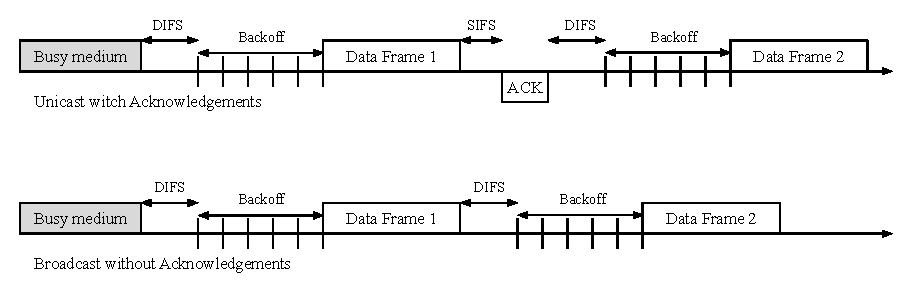
\includegraphics[scale=0.75]{figures/CSMA_CD.pdf}
	\caption{CSMA/CA with and without Acknolegements}
	\label{fig:CSMACD}
\end{figure}

Before a station transmitts data it has to check or listen to the medium to avoid collisiion resulting in packet loss.
Only when the medium is free, the station waits for a \ac{DIFS} and a random backoff.
The backoff is a random time within a \ac{CW} to prevent all stations from transmitting immediately after the \ac{DIFS}.
The \ac{CW} consists of several slots, each consisting of 20$\mu$s in 802.11b.
If a transmission was not successful, the station doubles the \ac{CW}, 
this doubles the average waiting time and is intended to prevent re-collisions.
The minimum \ac{CW} in 802.11b is set to 16 slots.

\subsection{Data Link Transmissions}

When packets are sent on the data link layer, they do not contain the headers to the layers above, such as TCP/IP.
Therefore, IP addresses cannot be used to transmit packets to another network.
There are three basic types of data link transmissions: unicast, broadcast and multicast.

\subsubsection*{Unicast}

The link layer unicast is used to send data over an single hop to the target \ac{WES} destination.
The link layer of each \ac{WES} checks the destination MAC address in the link layer header and 
discards the frame if the destination address does not match its own address.
It is therefore a direct communication between the transmitter and the WES.

Unicast is by default reliable.
When the Unicast reaches the destination \ac{WES} an acknowledgement frame is send back after the \ac{SIFS} + backoff.\todo{when to explain CSMA/DC?}
If the acknowledgement is not successfully received by the sender, the sender will repeat the transmission for a given number.
When the number is exceeded, the packet could not be delivered. 
If the number is set to zero, the unicast can be considered as non-reliable.
\TODO{example}

\begin{figure}[h]
	\centering
	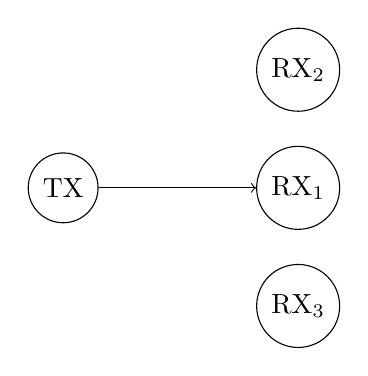
\begin{tikzpicture}[node distance={15mm}, main/.style = {draw, circle}] 
		\node[main] (1) 				{TX}; 
		\node[main] (2) [right=0cm and 2cm of 1]	{$\text{RX}_1$}; 
		\node[main] (3) [above of =2]				{$\text{RX}_2$}; 
		\node[main] (4) [below of =2]				{$\text{RX}_3$}; 
		\draw[->] (1) -- (2);
	\end{tikzpicture} 
	\caption{Unicast Transmission}
	\label{fig:unicast_topology}
\end{figure}

\subsubsection*{Broadcast}

If a packet should be received from all \ac{WES}'s it can be distributed as broadcast.
The \ac{MAC} address of the destination address in the link layer is set to the common broadcast address, which is ff:ff:ff:ff:ff:ff.\\
In contrast to unicast, broadcast is not reliable. 
This is mainly because the packet is addressed to all nodes at the same time, and if link layer acknoledgements would be used, 
the acknoledgements would be sent by all nodes at the same time, 
because there is no mechanism in which order acknoledges should be answered. 
In addition, the sender of a broadcast does not know how many WESs he is addressing the packet to in the first place.
Retransmitting acknoledgements would lead to massive collision and loss of acknoledgements.
E.g. management information in a \ac{WLAN} is sent in a broadcast mode, because it has to reach every \ac{WES} and isn't worth to be acknoleged.

\begin{figure}[h]
	\centering
	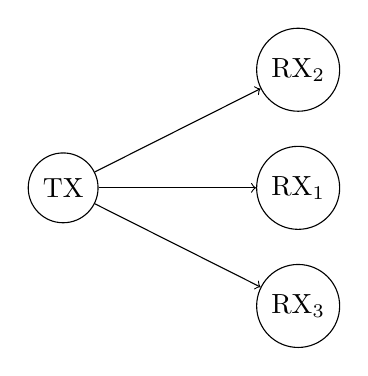
\begin{tikzpicture}[node distance={15mm}, main/.style = {draw, circle}] 
		\node[main] (1) 				{TX}; 
		\node[main] (2) [right=0cm and 2cm of 1]	{$\text{RX}_1$}; 
		\node[main] (3) [above of =2]				{$\text{RX}_2$}; 
		\node[main] (4) [below of =2]				{$\text{RX}_3$}; 
		\draw[->] (1) -- (2);
		\draw[->] (1) -- (3);
		\draw[->] (1) -- (4);
	\end{tikzpicture} 
	\caption{Unicast Transmission}
	\label{fig:unicast_topology}
\end{figure}

\subsubsection*{Multicast}

\TODO{Mutlicast explain multicast mac address}
When the same packet should be transmitted to multiple \ac{WES}'s, but not to all, multicast can be used.
Transmitting the same packet multiple times via unicast is wasteful.
There are different approaches to realize acknowledgements for mutlicasts, they differ mainly by the respective field of application.
\TODO{examples for multicast ack + related work}
Level 2 multicast is often used for large files in audio or video streams, where a big amount of data is distributed and multiple clients listen simultaneously.

\begin{figure}[h]
	\centering
	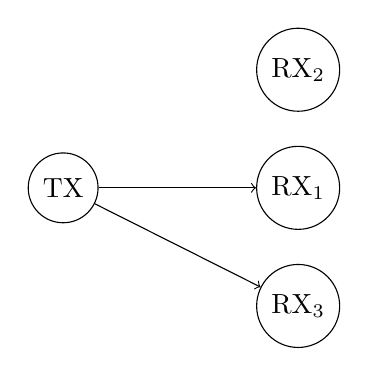
\begin{tikzpicture}[node distance={15mm}, main/.style = {draw, circle}] 
		\node[main] (1) 				{TX}; 
		\node[main] (2) [right=0cm and 2cm of 1]	{$\text{RX}_1$}; 
		\node[main] (3) [above of =2]				{$\text{RX}_2$}; 
		\node[main] (4) [below of =2]				{$\text{RX}_3$}; 
		\draw[->] (1) -- (2);
		\draw[->] (1) -- (4);
	\end{tikzpicture} 
	\caption{Unicast Transmission}
	\label{fig:unicast_topology}
\end{figure}
\todo{complete figure MC}


\section{Light protocols}

There are several lighting protocols that are used. The field of application ranges from wired CAN buses over ethernet cables to wireless WLAN networks.
To give a short insight, some of the most important protocols are explained below.

\subsection{DMX-512A}
\ac{DMX} 512A, is the current industry standard for stage lighting. It is based on \ac{CANproto}, therefore it uses wires.
Physically is the DMX protocol transmitted over a differential pair of lines using the RS-485 voltage levels. 
The bus signal is updated with 44Hz.
According to the specification are XLR-5 type connectors are to be used. \todo{image der connectoren}

\TODO{Show Hardware e.g. DMX Plug}

The endsystems are called fixture because it's most likely a lighting installation which is mounted somewhere, 
this could be a moving-head, fresnel, spotlight, stroboscope or any other light installation.
It could also be a fog machine that emits fog on an appropriate signal.

All devices are daisy chained together visualized in \ref{fig:dmx_diagram}.
The DMX controller is in the begin of each chain.
The receiving endsystems, are chained behind each other from output to input. 
A terminator, specified in the DMX specification, is to be connected to the final output.
 
\begin{figure}[h]
	\centering
	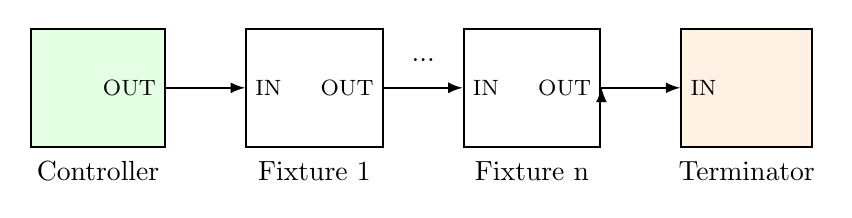
\begin{tikzpicture}[thick,
	    TFblock/.style= {
	        draw,  
	        minimum size=1.5cm}]
	
		% Blocks
		\node [TFblock,fill=green!10] (a) {\footnotesize{\ \ \ \ \ \ \ \ OUT}};
		\node [TFblock,fill=white!20,] (b) [right= of a] {\footnotesize{IN\ \ \ \ \ OUT}};
		\node [TFblock,fill=white!20] (c) [right =of b] {\footnotesize{IN\ \ \ \ \ OUT}};
		\node [TFblock,fill=orange!10] (d)[right =of c] {\footnotesize{IN\ \ \ \ \ \ \ \ \ \ \ \ }};

		% % Arrows
		\draw[-latex] 
		    (a.east) edge (b.west)
		    (b.east) edge (c.west)
		    (c.east) edge (d.west) ;

		% Labels
		\node[below=0.8cm] at (a){Controller};
		\node[below=0.8cm] at (b){Fixture 1};
		\node[below=0.8cm] at (c){Fixture n};
		\node[below=0.8cm] at (d){Terminator};
		\node[above=0.2cm] at (barycentric cs:b=1,c=1){ ... };

	\end{tikzpicture}
	\caption{Block Diagram of an DMX Universe}
	\label{fig:dmx_diagram}
\end{figure}

The hole chain is called DMX-Universe and can contain a set of 512 channel.
If there is a need of more channels one needs more DMX universes - each channel consists of one byte.
Due to the fact that a DMX universe always has its own bus, starting from a new controller can lead to inconveniences.

A channel in the event technology is to distinguish between e.g. a WiFi channel.
Each endsystem is assigned at least one, but usually several channels.
Every endsystems knows which channel is intended for it, this must to be preset.

For example: An RGB-LED spotlight could have three channels, one for each color.
Due to the resolution of one byte, the individual colors can (theoretically) be controlled in 256 different intensities.
If the Channel 0-56 are already used, it could be set to channel 57, 58, 59.
Any other free channel range would also be possible, provided it is connected.
There exist hardware with automatic-address-assignment.

\TODO{Image of fixtures distributed on channel}

Since \ac{DMX} is unidirectional it can be assumed that the endsystems generally only receive or forward (daisy chain) control signals sent from the control console.
This is a major limitation of DMX, beside of the rather small universe size.
It is also not reliable, the use of fire installations is therefore considered too dangerous.

\subsection{Art-Net}
\label{sec:artnet}
\begin{itemize}
	\item Example of an wifi protocol
	\item 2.4 or 5GHz
	\item DMX-Like
	\item related work
\end{itemize}

Due the limitation of 512 channel for each universe there where protocols implemented using the 
Art-Net also called Art-Net DMX is 

\section{ESP Platform}

Almost every 802.11 capable \ac{MCU} could be picked for this research.
But there are several reasons why the ESP Platform from Espressif is a valid choice.
There are several chips provided by Espressif with WiFi specifications, these chips are very affordable (\todo{TOLJA: ESP32 Kosten in € 2021 aufführen? Link? Datum?}) 
and althrough the ongoing chip crysis (2021) there are easy to get, in contrast of the also very popular Chips from the manufacturer Arduino, which are also more expansive.
Espressif supports an own development IDF to flash the chips, with minor tweeks it's also to use the Arduino IDE.\\
However the properitary protocol ESP-Now which, just supported in the ESP Ecosystem, is discussed below \cref{sub:ESP-Now} 
and has promising properties for a solid and fast realisation of a low level protocol.
\TODO{paper about esp above arduino}

\subsection{ESP32 Hardware}

The chip ESP32 is quite common in DIY projects around everything from home automation to light installations 
and can baught on development boards, which are ready to use.
The chip \ref{fig:esp32} is promoted with several features: \todo{this is cited from: link zum esp32 datasheet}
\begin{itemize}
	\setlength\itemsep{-0.0em}
	\item Fast CPU (2 cores at 240 MHz)
	\item 802.11 b/g/n with up to 150 Mbps (2.4GHz)
	\item Wifi Multimedia (WMM)
	\item Immediate Block ACK
	\item Automatic Beacon monitoring (hardware TSF)
	\item Virtual Wi-Fi Interfaces
	\item Simultaneous support for Infrastructure, SoftAP, and Promiscuous modes
	\item Bluetooth v4.2 BR/EDR and Bluetooth LE
	\item Advanced Peripheral Interfaces: GPIO, ADC, DAC, touch sensors, hall sensor, 
	SPI, I2S, I2C, UART, CAN, RMT (TX/RX), Motor/LED PWM 
\end{itemize}

\begin{figure}[h]
	\centering
	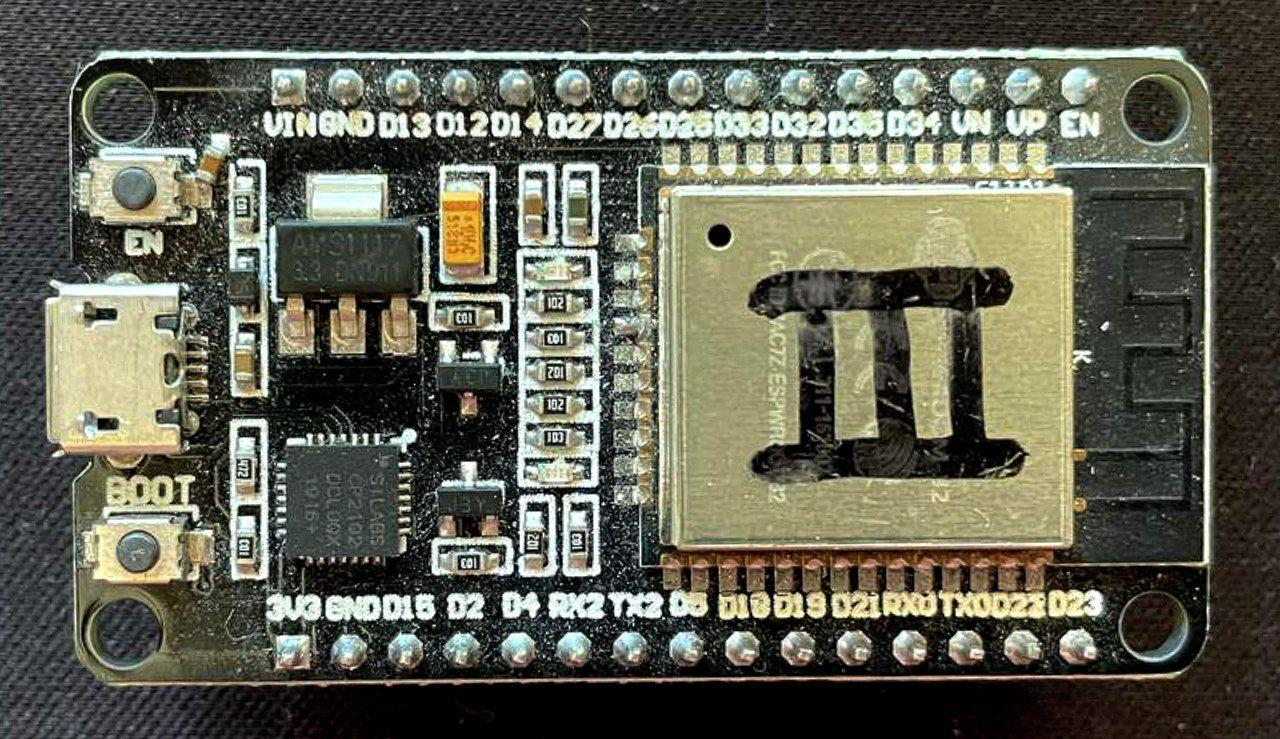
\includegraphics[scale=0.2]{figures/espdevboard.jpg}
	\caption{ESP32 Devboard (Devkit V1)}
	\label{fig:esp32}%
\end{figure}

\TODO{final words to the ESP32 Hardware - a lot of features for a cheap hardware}

\subsection{ESP-Now}
\label{sub:espnow}
ESP-NOW is a properitary protocol developed by Espressif. 
ESP-NOW is widely used in smart light, remote controlling, sensor, etc\todo{cite ESP documentation website}. 
It is a conectionless protocol, so the \ac{WES}'s are in Ad-Hoc mode insted of \ac{STA}.
It is just supported on the ESP8266, ESP32 and ESP32s, all chipsets from Espressif, but they are compatible with each other.
Because of this, a ESP-Chip as gateway is needed to interact from the outside to the ESP-NOW communication. 

Through the hardware limitation of the boards it can just be used on the 2.4 GHz frequncy band.
ESP-NOW allows 10 ESPs for pairing with encryption and up to 20 without encryption.
Espressif promises throuput of up to 30MBit/s with and a possible range of up to 1km.
However \emph{\textcite{ESPNOWPaper}} measured a range of the unmodified onboard antenna of the ESP32 
and just got a \emph{\textcite{ESPNOWPaper} stable commication up to 190m in open field}.\\

The focus of the ESP-NOW protocol is on low power consumption.
A connectionless communication between \ac{WES}'s not only saves energy during the authentication process, 
Additionally, is the commonication the the properties of the ad-hoc mode, direct and not over a second access point.
The protocol has a limitation of a limeted payload of 250 byte for each transmission.
It also has a much less overhead, which results in shorter airtime, less disturbances and also less power consumption through the antenna 
(latter is not relevant for this thesis).
There is no TCP/IP header to be transmited. 
For very small payloads, this offset can become dispropotional.

The default ESP-NOW bit rate is 1 Mbps it uses a channelwidth of 20MHz, there is no double channel (40Mbit/s or higher) used.
But e.g. the low energy, high range protocol Long Range Wide Area Network (LoRaWAN) suffers from a to slow throuput for this application.

To undersant what ESP-NOW does it needs to take a look to the vendor-specific action frame transmiting ESP-NOW data. 
\todo{cite somehow the ESP-NOW documentation pdf: ESP-IDF Programming Guide: ESP-NOW, source: \url{https://docs.espressif.com/projects/esp-idf/en/latest/esp32/api-reference/network/esp_now.html}}
\TODO{Explain Vendor Specific Frames!}

% \url{https://www.heise.de/tipps-tricks/}

visualized in \ref{fig:esp-now_frame_format}.

\begin{table}[h]
	\centering
	\begin{tblr}{	hlines,
					vlines,
					rows = {ht=1.3cm},
					columns = {halign=c},
					colspec = {XXXXXX},} 
	\makecell{MAC\\Header} & \makecell{Category\\Code} & \makecell{Org.} & 
	\makecell{Random\\Values} & \makecell{Vendor\\Specific\\Content} & \makecell{FCS}\\
	\end{tblr}
	\begin{tabularx}{\linewidth}{ X X X X X X }
		\makecell{\footnotesize{24}} & \makecell{\footnotesize{1}} & \makecell{\footnotesize{3}} & 
		\makecell{\footnotesize{4}} & \makecell{\footnotesize{7 $\sim$ 255}} & \makecell{\footnotesize{4}} \\
	\end{tabularx}
	\caption{ESP-NOW Frame Format}
	\label{fig:esp-now_frame_format}
\end{table}

\begin{itemize}
	\setlength\itemsep{-0.0em}
	\item \textbf{MAC Header:} As ESP-NOW is connectionless, the MAC header differs from that of standard frames.
	\item \textbf{Category Code:} The Category Code field is set to the value(127) indicating the vendor-specific category.
	\item \textbf{Organization Identifier:} The Organization Identifier contains a unique identifier (0x18fe34), which is the first three bytes of MAC address applied by Espressif.
	\item \textbf{Random Value:} The Random Value filed is used to prevents relay attacks.
	\item \textbf{Vendor Specific Content:} The Vendor Specific Content contains vendor-specific fields (table \ref{fig:esp_now_vendor_format})
	\item \textbf{Frame Check Sequence:} Used for error correction in layer 2.
\end{itemize}

Inside of the ESP-NOW frame \ref{fig:esp-now_frame_format} is the vendor specific content visualized in \ref{fig:esp_now_vendor_format}. 

\begin{table}[h]
	\begin{tblr}{	hlines,
					vlines,
					rows = {ht=1.3cm},
					columns = {halign=c},
					colspec = {XXXXXX},} 
		\makecell{Element\\ID}& \makecell{Length} & \makecell{Org.\\Identifier} & \makecell{Type} & \makecell{Version} & \makecell{Body}  \\
	\end{tblr}
	\begin{tabularx}{\linewidth}{ X X X X X X }
		\makecell{\footnotesize{1}} & \makecell{\footnotesize{1}} & \makecell{\footnotesize{3}} & \makecell{\footnotesize{1}} & \makecell{\footnotesize{4}} & \makecell{\footnotesize{7 $\sim$ 250}} \\
	\end{tabularx}

	\caption{Vendor Specific Action Frame}
	\label{fig:esp_now_vendor_format}
\end{table} 

\begin{itemize}
	\setlength\itemsep{-0.0em}
	\item \textbf{Element ID:} The Element ID field is set to the value (221), indicating the vendor-specific element.
	\item \textbf{Length:} The length is the total length of Organization Identifier, Type, Version and Body.
	\item \textbf{Organization Identifier:} The Organization Identifier contains a unique identifier(0x18fe34), which is the first three bytes of MAC address applied by Espressif.
	\item \textbf{Type:} The Type field is set to the value (4) indicating ESP-NOW.
	\item \textbf{Version:} The Version field is set to the version of ESP-NOW.
	\item \textbf{Body:} The Body contains the ESP-NOW data.
	\todo{this is cited from espressif manual!!}
\end{itemize}

It is worth to mention, that the vendor specific content \ref{fig:esp-now_frame_format} is allowed to contain up to 255 byte,
but the sum over all values in \ref{fig:esp_now_vendor_format} if the body would contain the maximum of 250 bytes, 
leads to a total of 260 bytes.\todo{255 != 250 is it really that important?}
The values are from the documentation of ESP-NOW from Espressif.
They also claim, that broadcast is not supported in ESP-NOW, but it is.
It seems that the documentation isn't complitly finished (or translated).

\subsection{ESP-Now vs Art-Net Baseline}
\todo{subsection can be on a wrong position!}
\TODO{remove newpage command}
\begin{itemize}
	\item Network stack diagram
	\item baseline
\end{itemize}

\TODO{ESP-NOW Baseline Artnet should be moved to Design part??}

\chapter{Proposed Approach}

% \begin{itemize} 
% 	\item describe everything you yourself did (as opposed to the fundamentals chapter, which explains what you built on)
% 	\item start with a theoretical approach    
% 	\item describe the developed system/algorithm/method from a high-level point of view
% 	\item go ahead in presenting your developments in more detail  
% 	\item recommended length: approximately one third of the thesis.
% \end{itemize}

Different approaches are presented and discussed in this chapter using data link unicast or broadcast in different specifications,
these were also empirically tested and evaluated in the \cref{sec:evaluation}.
At the end of this chapter, the test setup will be introduced and 
it is briefly explained how the chips are programmed.

\section{Design}

\begin{table}[h]
	\centering
	% \label{tab:layer_overview}
	\begin{tabular} { ccc }
		\begin{tabular}{ |c| } 
			\hline
			Art-Net\\
			\hline
			UDP\\
			\hline
			IP\\
			\hline
			802.11 DL/Unicast\\
			\hline
			802.11* PHY\\ 
			\hline
		\end{tabular}
		\begin{tabular}{ |c| } 
			\hline
			Slim Application\\
			\\
			\\
			\hline
			802.11 DL/UC or BC\\
			\hline
			802.11* PHY\\ 
			\hline
		\end{tabular}
	\end{tabular}
	\caption{Art-Net Layer compared with Slim Data Link Layer}
	\label{tab:Layer}
\end{table}

The use of high-layer protocols, such as Art-Net \cref{sec:artnet}, in lighting technology involves a considerable overhead. 
Because the lighting console does not talk directly to the \ac{WES}, communication must be controlled via an \ac{AP}, 
which means that the \ac{IP} (layer 3) must be used for addressing and \ac{UDP} (layer 4) for transporting the data. 
They both come withe additional headers. 
Such an overhead can lead to latency, channel congestion and packet loss.
 
In an ad-hoc network \cref{itm:bss}, on the other hand, packets can be sent directly on the MAC (layer 2) \cref{tab:Layer}. 
With a payload of a few bytes to each WES, keeping overheat small can be quite important. 
Complexity problems as often typical in Ad-Hoc networks are not to be assumed, 
since the controller at the light desk must normally stand in line of sight to the individual WES, 
from there finally the lighting technician from there must have everything in the range of vision to be able to intervene. 
One can therefore assume a simple star topology.
In the following the ESP-NOW \cref{sub:espnow} protocol was chosen to distribute the packets low-level, 
because even if it was not developed for this purpose the specification fits quite well to the requirements.

\todo{topology of data flow isnt linked in the text}
\begin{figure}[h]
	\centering
	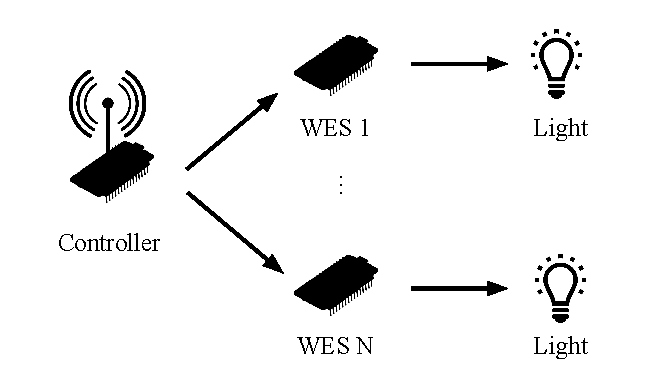
\includegraphics[scale=0.75]{figures/dataFlow.pdf}
	\caption{Topology of the Data Flow}
	\label{fig:testbed}
\end{figure}

For the purpose of this analysis, the controller transmits 20 Byte (analogue to 20 DMX channels) to every WESs.
Four different metrics are considered, which where discussed in the requirements.
\begin{itemize}
	\item \textbf{Latency} \\
	What is the latency from commanding the controller to the estimated reaction at the WES e.g. lighting of a light?
	For the sake of simplicity, delays caused by the microcontroller instruction set, data distribution and 
	control of the light installation are neglected and the focus is placed only on the airtime.
	Low latency is important so that the lighting technician can intervene live in the light show,
	but the lights do not react with delay.
	\item \textbf{Update Frequency}\\
	How often can the we update all WESs per second? 
	This results in how smooth movement of moving heads are moving or how smooth the transition
	of the color of an LED can be performed
	and the control can be adapted rhythmically to the musical beat.
	\item \textbf{Reliability}\\
	Wie sicher kommen die vom Controller gesendeten Daten bei den WESs an?
	Lack of reliability can result 
	in two WESs positioned next to each other not behaving the same because one of them only receives half of the signals.
	\item \textbf{Synchronisation}\\
	Are the signals sent to different WESs carried out at the same time?
	If two of the WESs are to be controlled simultaneously, 
	but the signal was transmitted one after the other, they have to wait for each other so that the lights change at the same time.
\end{itemize}

\subsection*{Slim Unicast}

The implementation that probably comes closest to Art-Net's is to replace the TCP packets sent by Art-Net 
to the respective IP-Address of the WESs with unicasts to the MAC-address of the WES.
Of course, the MAC address of all WESs must be known and they must all be paired with the controller, but 
this process is just analogous to  mapping the corresponding IP addresses after dialing the WESs into a WLAN.

\subsubsection*{Latency}

Latency describes the time between a command and the expected response, here considered as airtime.
The airtime using 1Mbit/s is rather easy calculated, every Byte (8 Bits) takes 8$\mu$s.

For a full transmission the PHY and MAC preamble and header be transmitted twice, once for the data and once for the acknowledgement.
The MAC body contains the payload, which depends of the needs of the addressed \ac{WES}.
In a perfect clean channel the sender hasn't to defer, but has to take a \ac{DIFS} plus a backoff.
A perfect empty channel resets the CW to CW$_{min}$, which are 31 slots in 802.11b
and a slot time of 20$\mu$s an average delay of $370\mu$s is estimated.

\begin{align}
	\frac{CW_{min}}{2}=\frac{31}{2}=16.5 \\
	20\mu s \cdot 16.5 = 370\mu s
\end{align}

\begin{table}[h]
	\centering
	\begin{tabular} { lrr }
		\toprule
		\multicolumn{1}{c}{Frame segment}
		& \multicolumn{1}{c}{Byte}
		& \multicolumn{1}{c}{Duration in $\mu$s} \\
		\midrule
		DIFS								& -		& 50 \\
		Average Backoff						& -		& 370 \\
		PHY header: PLCP preamble			& 18	& 144 \\
		PHY header: PLCP header				& 6 	& 48 \\
		MAC headers							& 28	& 224 \\
		MAC body							& 20 	& 160 \\
		\textbf{= tx time data}				& 		& \textbf{956} \\
		SIFS								& -		& 10 \\
		PHY header: PLCP preamble			& 18	& 144 \\
		PHY header: PLCP header				& 6		& 48 \\
		MAC headers, no MAC body	 		& 18	& 112 \\
		\textbf{= tx time ack}				& 		& \textbf{314} \\
		\bottomrule
	\end{tabular}
	\caption{Composition of the Total Airtime (tx + ack)}
	\label{tab:airtime_unicast_calc}
\end{table}

The total airtime of the transmission of data and ack, assuming the transmission arrived successfully, is $t_tx=1100\mu$s.
Strictly speaking, the light could also be changed before the acknolegement is sent, i.e. after 956$\mu$s.
The latency scales linearly, the delay to the n-th WES is:
\begin{align}
	\text{Airtime} = N \cdot t_{tx} = N \cdot 1270\mu s
\end{align}

In order to avoid unnecessary load on the radio channel, Art-Net transmit only the changes.
In the worst case, however, changes affect all WESs at the same time.

\subsubsection*{Update Frequency}
Following the approach of DMX and updating the 'bus' every 44Hz, would made by sending the packets round robin via unicast. 
With a correspondingly high number of WESs, this could be challenge with a transmission speed of 1MBit/s, 
it also scales linearly with each additional WES. 
In an labor steril empty channel, denying all side latencys, there airtime could be for N WESs:
\begin{align}
	\text{Frequency} = \frac{1}{N \cdot 1270\mu s} = \frac{787.4}{N} Hz
\end{align}

For 10 WESs, addressed with respectively 20 Byte, it would still be 787.4 Hz.
This is far above the update frequency of DMX with 44Hz, but also very unrealistic and just intended to show,
that it could theoretically be within the realm of possibility.

\subsubsection*{Reliability}

A benefit of the unicast is the support of acknoledgements. 
The acknoledgements trigger a retransmission if no packet has arrived, therefore a controlled light will receive its signal in any case.
So the reliability should be very good.

\subsubsection*{Synchronisation}

Synchronising the unicast transmissions costs a lot of 
latency, through buffering delay.
This is because not only does each WES have to wait until its own packet has arrived,
but until all the packets have arrived at all WESs.
The implementation is chosen in such a way that each WES knows at which position of the round-robin it is
and delays the execution of the successfully received transmission until the last WES has also received its signal.
The delay must then be calculated deterministically.
In ESP-NOW, the default is set to 8 retransmissions, so in the worst case it is assumed that a packet is sent 8 times
and that for each WES.

\begin{align} 
	\text{Airtime}_{sync} &= 8 \cdot N \cdot 1270\mu s = N \cdot 10160\mu s \\
	\text{Frequency}_{sync} &= \frac{1}{N * 10160\mu s} = \frac{98.42}{N} Hz
\end{align} 

The idea of the slim unicast is, that a transmission to each device is very fast, because the transmitted payload small.
However, since we are sending many small packets, it can be assumed that we will be sending a lot of overhead.
So it's playing off reliability against transmission speed.
It can be said that synchronisation is a feature that should be dispensed with in the slim unicast for the sake of latency.
An approach that has not been explored is to reduce the number of retransmissions.

\subsection*{Slim Broadcast}

The ESP-Now protocol supports both unicast and broadcast.
Instead of transmitting every unicast after each other, 
Slim Broadcast transmitts a broadcast with the payload of all channels at the same time to all fixtures.
If there is a need for more than 250 Byte (DMX channel) a second broadcasts has to be send to transmit containing the missing data.
To achieve this, each WES must be told in advance at which position in the payload its data is located.
The broadcast must also spend one byte of payload for the sequence number.
Only in the application layer do the WESs discard the incorrect broadcasts and read out their area from the entire payload.

For the unicast the payload was assumed to be 20 byte for each WES, the same amount is assumed for each WES in the Slim Broadcast calculations.
The maximum payload of the broadcast is reduced to 200 byte, instead of the possible 250 bytes, 
because when it is close to the 250 byte limit, reliability is supposed to collapse.
\todo{cite something 250 byte max payload ESPNOW}

\subsubsection*{Latency}

The latency of the broadcast is easier to calculate than that of unicast, because the acknoledgments are no longer necessary.
In return, the payload of a single transmission increases.
Assuming 10 WESs are to be addressed, each with 20 byte payload \ref{tab:airtime_broadcast_calc}.

\begin{table}[h]
	\centering
	\begin{tabular} { lrr }
		\toprule
		\multicolumn{1}{c}{Frame segment}
		& \multicolumn{1}{c}{Byte}
		& \multicolumn{1}{c}{Duration in $\mu$s} \\
		\midrule
		DIFS								& -		& 50 \\
		Average Backoff						& -		& 330 \\
		PHY header: PLCP preamble			& 18	& 144 \\
		PHY header: PLCP header				& 6 	& 48 \\
		MAC headers							& 28	& 224 \\
		MAC body							& 200 	& 1600 \\
		\textbf{= tx time data}				& 		& \textbf{2456} \\
		\bottomrule
	\end{tabular}
	\caption{Composition the Broadcast Airtime}
	\label{tab:airtime_broadcast_calc}
\end{table}

\begin{figure}[h]
	\centering
	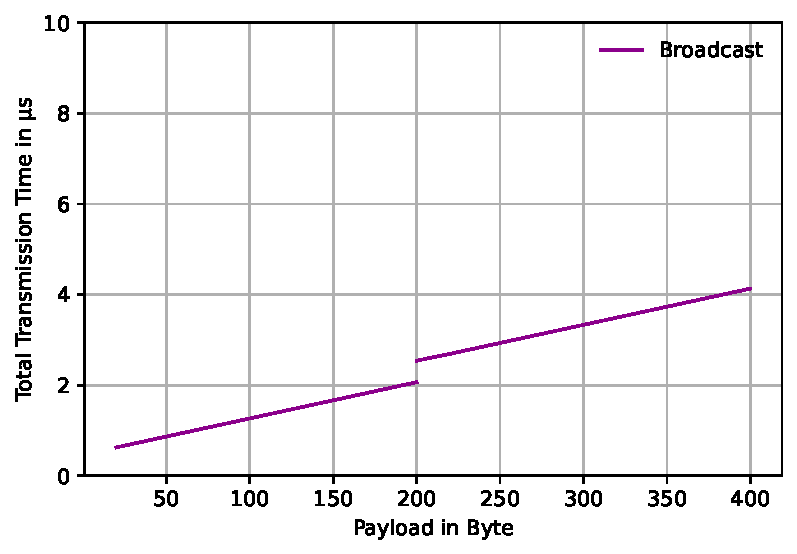
\includegraphics[scale=0.6]{/home/walther/Documents/bachelor/Plot2/Graphs/bc_analytic.pdf}
	\caption{Transmission Time of Broadcasts Depending on Payload}
	\label{fig:bc_analytic}
\end{figure}

Due to the fact that a second broadcast is needed if the maximum payload of ESP-NOW is exceeded,
the expected transmission time is not continuous, as shown in \cref{fig:bc_analytic}.
It is easy to see that the additional overhead caused by adding another package creates noticeable latency.

\subsubsection*{Update Frequency}

However, while compareing this to the latency of unicast \ref{tab:airtime_unicast_calc},
it becomes clear that the low overhead and the missing acknoledgements lead to a significantly higher rate.
A complete pass, i.e. addressing all WESs with 20 bytes, is already an order of magnitude faster from a number of 10 WESs.

\begin{align}
	\text{Frequency}_{UC} &= \frac{1}{10 \cdot 1270\mu s} = 78.7 Hz \\
	\text{Frequency}_{BC} &= \frac{1}{2456\mu s} = 407.2 Hz
\end{align}

Even if these values are only remotely comparable with real measurement data, it is clear,
that the throughput is significantly higher with broadcast than with unicast.
This effect should be even clearer under real conditions.

\begin{figure}[h]
	\centering
	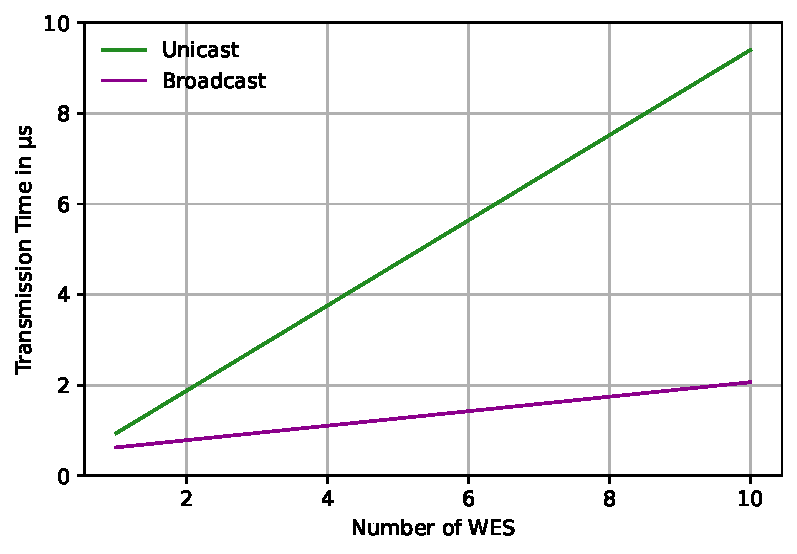
\includegraphics[scale=0.6]{/home/walther/Documents/bachelor/Plot2/Graphs/bc_uc_transmissiontime_analytic.pdf}
	\caption{Transmission Time of Unicast vs Broadcast}
	\label{fig:bc_uc_transmissiontime_analytic}
\end{figure}

\subsubsection*{Reliability}

The huge advantage that the Slim Broadcast has over the Slim Unicast in terms of update frequency,
comes at the cost of lower reliability.
Broadcasts can't do acknolegements,\todo{ref to fundamentionals, datalink, broadcast}
a WES that has poor reception to the controller, will not receive packets and the controller cannot take countermeasures.
\cref{sec:DLbroadcast}

\subsubsection*{Synchronisation}
Insead of transmitting to several fixtures after each other slim broadcast just transmitts to all fixtures at the same time.
This solves the problem of synchronization for less than 200 channel.
For more than 200 each WES has to wait until the last broadcast has arrived.
In contrast to unicast, the buffering delay can be calculated almost deterministically for broadcast 
due to the absence of automatic retransmissions.

\subsection*{Rapid Repetition}

\todo{Is Rapid Repetition a appropriate name? Unsosliced Repetition is better siehe Paper?}

To improve the reliability of the slim broadcast, the same transmission can simply be repeated unsolicited.
The idea is not to wait for a missing acknolegedment, but to increase the probability that one of the packets got through.
\todo{Cite paper A First Implementation and Evaluation of the IEEE 802.11aa Group Addressed Transmission Service}
The reliability of the Slim Broadcast with Rapid Repetition is improved with every rapid repetition (RR).
In the formula below \cref{math:rr_sr}, with RR set to zero, there happens no repetition.

\begin{figure}[h]
	\centering
	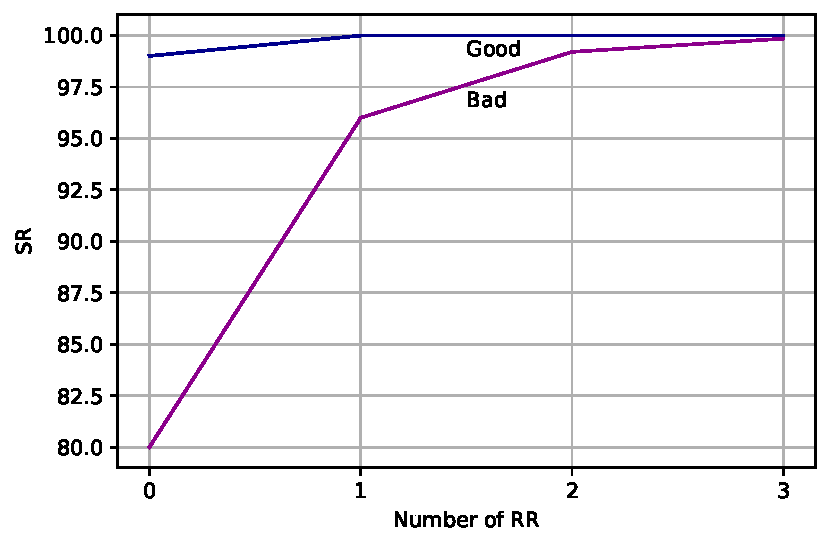
\includegraphics[scale=0.6]{/home/walther/Documents/bachelor/Plot2/Graphs/theory_sr_rr.pdf}
	\caption{Success Ratio increase with increasing number of RR}
	\label{fig:theory_rr_sc}
\end{figure}

\begin{align}
	\label{math:rr_sr}
	\text{SR}_{RR}(RR)	&= 1-(1-\text{SR})^{RR+1} \\
	\text{SR}_{RR}(0) 	&= SR \\
	\text{SR}_{RR}(1) 	&= 1-(1-\text{SR})^{2}
\end{align}

The RR makes it possible to reach WESs with poor reception much more reliably,
However, WESs that have very good reception also receive the same packet redundantly.
The update frequency of a BC with RR must be divided by the number of repetitions, compared to one without repetitions,
the same applies to the latency when synchronisation is required.
However, in contrast to unicast, broadcast offers such shorter transmission times,
that at least a few repetitions can be accepted. \cref{fig:rr_analytic}

\begin{figure}[h]
	\centering
	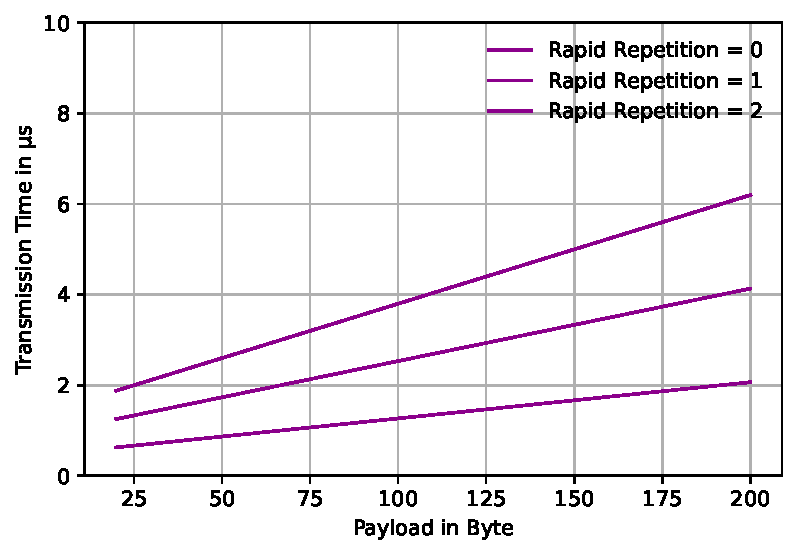
\includegraphics[scale=0.6]{/home/walther/Documents/bachelor/Plot2/Graphs/rr_transmission_time.pdf}
	\caption{Transmission Time with with different sets of RR over rising Payload}
	\label{fig:rr_analytic}
\end{figure}

\subsection*{Delayed Rapid Repetition}
\label{sub:DelayedRepetition}

To push the idea of rapid repetion even further, should also temporarily occuring noise be taken into account.\todo{displaced repetition vs delayed repetition}
This can cause all the repetitions to be captured at once.
If the individual repetitions of the first sequence are sent displaced together with those of the second sequence,
then the probability that at least one of the repetitions is not detected by a occuring noise noise is increased.

By staggering the individual sequences, the update frequency is not affected,
because just as many packets are sent as with Slim Broadcast RR.
The latency, on the other hand, is significantly increased, especially when synchronisation is maintained.
In the given example of \cref{fig:badChannel} the WESs has to wait for 5 times the duration of a broadcast transmission, instead of three.

\begin{figure}[h]
	\centering
	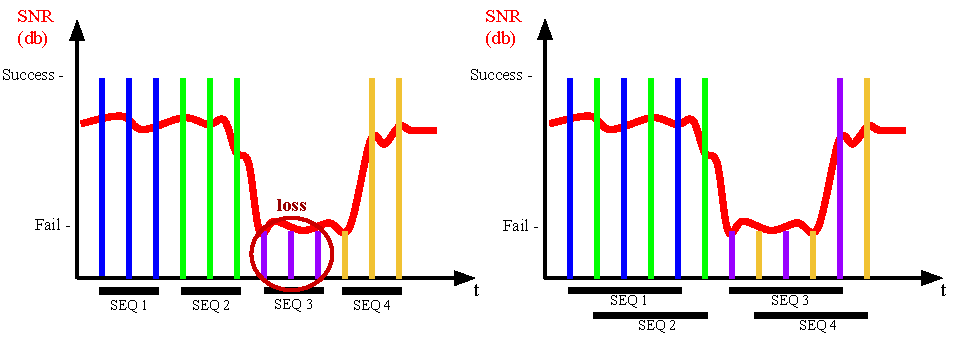
\includegraphics[scale=0.75]{figures/BadChannel.pdf}
	\caption{Rapid Repetition = 3 over a occuring noise}
	\label{fig:badChannel}
\end{figure}

The delay of the Delayed Rapid Repetition (DR) can also be extended considerably.
In extreme cases, it could be set to the number of sequences, which is of course impractical,
but interleaving two or three sequences could help counteract persistent noise.

\begin{figure}[h]
	\centering
	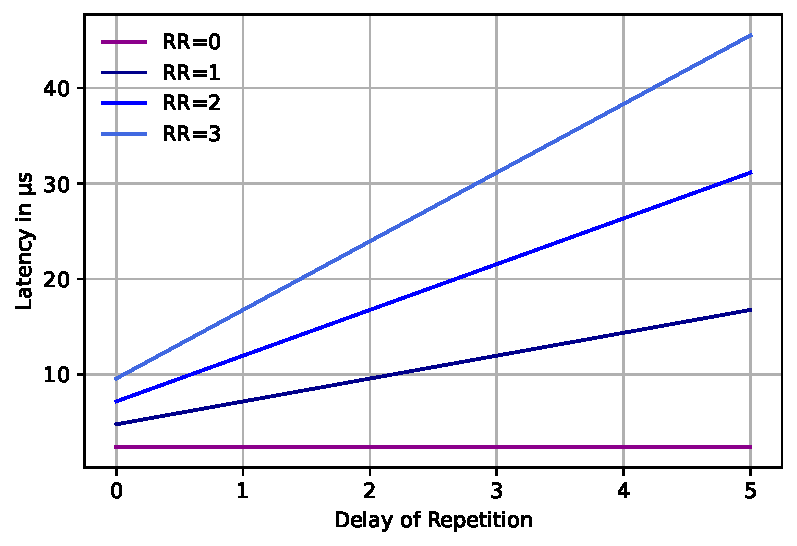
\includegraphics[scale=0.60]{../Plot2/Graphs/bc_dr.pdf}
	\caption{Latency of DR, transmitting 200 Byte}
	\label{fig:dr_delay}
\end{figure}

With DR, improved reliability comes at the cost of latency, not update frequency,
because no more packets are sent, only the order is shifted.
If no repetition is applied, the delayed rapid repetition has no influence,
which is why the graph \cref{fig:dr_delay} remains constant for RR=0.
The greater the RR and the delay of the DR, the more packets where send
between the first and the last packet of each sequence.

The measurement results \cref{sec:evaluation} will show whether the use of delayed repetition 
can reduce the number of rapid repetitions while maintaining or even improving reliability.

\section{Implementation}

The developer boad ESP32 Devkit V1 used in the experiments (\cref{sec:evaluation}) for the collection of the data
can be ordered cheaply 
\footnote{3.79€, www.aliexpress.com, ESP32 Devboard V1, 3/3/22}
from common (most favourably Chinese) websites. 
The most accessible way to flash a chip is using the Arduino IDE, which can be easy configured for flashing ESPs.
A more precise approach is to use the IDF of Espressif itself, 
which can also be easily made to work by installing the toolchain and build tools and an Plugin for your favorite IDE.

\begin{figure}[h]
	\centering
	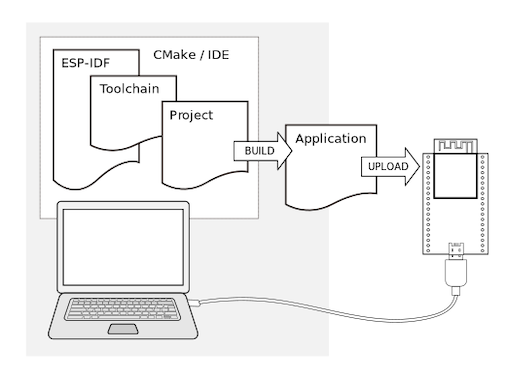
\includegraphics[scale=0.4]{figures/ESP-ISF.png}
	\caption{Flashing ESP}
	\label{fig:ESP-IDF}
	\footnote{\url{https://docs.espressif.com/projects/esp-idf/en/latest/esp32/_images/what-you-need.png, 3.3.2022}}
\end{figure}

Espressif has provided a user guide for the use of ESP-NOW ~\cite{ESPNOWGuide},
but unfortunately it contains some of informations which are outdated, 
for example, it claims that broadcast is not supported.
However, more detailed information can be found on the website.
% \footnote{\url{https://docs.espressif.com/projects/esp-idf/en/latest/esp32/api-reference/network/esp_now.html}}.

To use ESP-NOW on an ESP, only a few steps are necessary.
The chip must activate Wifi and put it in STA mode and ESP-NOW can be activated.
The two libraries "esp\_wifi.h" and "esp\_now.h" are required for this.

\begin{lstlisting}[caption=Init ESP-NOW]
WiFi.mode(WIFI_STA);
esp_now_init();
\end{lstlisting}
\label{lst:init}

\todo{check formatation in the final version}

Later, the individual MAC addresses of the WESs must be saved.
These are created in a separate header file and can then be added during the setup of the chip.
The MAC address is needed to add the respective WES to the peerlist.
However, the WES does not have to be switched on or within range for this, it is more a case of making the WES known to the controller.
The Controller can store up to 20 devices in his peerlist at the same time.

\todo{listing box prevent linebreaks on newpage}
\begin{lstlisting}
#ifndef MACLIST_H
#define MACLIST_H

uint8_t WES_MAC_1[6] = { 0xFC ,0xF5 ,0xC4 ,0x31 ,0x9A ,0x44 };
uint8_t WES_MAC_2[6] = { 0x24, 0x0A, 0xC4, 0x61, 0x19, 0x08 };
uint8_t BC_MAC[6]    = { 0xFF, 0xFF, 0xFF, 0xFF, 0xFF, 0xFF };
\end{lstlisting}
\label{lst:macaddress}

\begin{lstlisting}[caption=Add Peers]
#include "maclist.h"

if (!esp_now_is_peer_exist(WES_MAC_1)) {
  peer_info.channel = 13;                   // 1-14
  memcpy(peer_info.peer_addr, WES_MAC_1, 6);
  esp_err_t status = esp_now_add_peer(&peer_info);
}
if (ESP_OK == status) {                     // check success
  Serial.println("[OK] Slave-peer added"); 
}
\end{lstlisting}

Sending an ESP-NOW unicast is performed with the method esp\_now\_send().
The MAC address of the recipient is passed, a pointer to the payload to be transmitted and its length.
In the case of a broadcast, the address field is filled with the broadcast address ff:ff:ff:ff:ff:ff),
The function esp\_now\_register\_send\_cb can be used to check whether the cast was successfully sent out.
It is important to write as little code as possible in such a callback function.
If you send the next package only after receiving the dispatch confirmation, then you can be sure that the packages are sent in the correct format,
that the packages are sent in the correct order.

\begin{lstlisting}[caption=Send ESP-NOW Cast UC/BC]
void metaInformationToSlaves(const uint8_t *peer_addr, struct_advanced_meta metaData) {
  esp_now_register_send_cb(onDataSent);     // register callback

  esp_err_t status = esp_now_send(WES_MAC_1,
                                 (uint8_t *) &payload,
                                 sizeof(payload));
  if (ESP_OK == status) {                   // check success
    Serial.println("[OK] ESP-NOW sending"); 
  }

void onDataSent(const uint8_t *mac_addr, esp_now_send_status_t status) {
  if (status == ESP_NOW_SEND_SUCCESS) {
    Serial.println("[OK] ESP-NOW Send"); 
  }
}
\end{lstlisting}
\label{lst:sendcast}

Working with mirocontrollers requires a non continous program-flow, instead it's event-based.
For the individual WESs, a callback function is registered after setup, 
it's called when an ESP-NOW transmission is passed on to the application layer.

\begin{lstlisting}[caption=ESP-NOW Callback Functions]
esp_now_register_recv_cb(OnDataRecv);

void OnDataRecv(const uint8_t *mac_addr, const uint8_t *incomingData, int data_len) {
  if (incomingData[0] == 253) {             // setup data
    applyMetaInformation(incomingData, data_len);
    return;
  }
  if (incomingData[0] == 255) {             // verify data
    applyPayload(incomingData, data_len);
  }
  if (incomingData[0] == 254) {             // return results
    sendResultsToMaster();
    return;
  }
\end{lstlisting}
\label{lst:callback}



\chapter{Evaluation}
\label{sec:evaluation}
% \begin{itemize}
% \item measurement setup / results / evaluation / discussion
% \item whatever you have done, you must comment it, compare it to other systems, evaluate it
% \item usually, adequate graphs help to show the benefits of your approach
% \item each result/graph must not only be described, but also discussed (What's the reason for this peak? Why have you observed this effect? What does this tell about your architecture/system/implementation?)
% \item recommended length: approximately one third of the thesis.
% \end{itemize}

\section{Methodology}
One challenge in programming the controller and the WESs,
is the state-based approach and the fact that the WESs can only communicate restricted to each other.
There were therefore two types of state machines, one for the controller and one for the WESs.

The testbed \cref{fig:testbed} is set up that the PC is connected to the microcontroller via wired \ac{UART}, this microcontroller is the controller.
The controller then communicates exclusively via ESP-NOW with the WESs,
these then control in different ways with the stage lights and motors.
The WESs never respond to the controller for the actual application, the communication is unidirectional.
However, in order to evaluate the test data, the WESs are put into a mode in which they send the data to the controller, also via ESP-NOW.
From there, they are also sent to the PC via UART.

\begin{figure}[h]
	\centering
	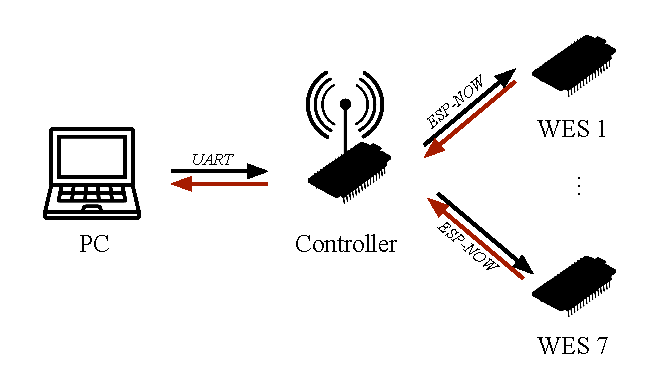
\includegraphics[scale=0.75]{figures/TestFlow.pdf}
	\caption{Data Flow for Measurement}
	\label{fig:testbed}
\end{figure}
\todo{change N to the actual number of WESs = 7}

The experiment is started from the PC, a JSON is then transmitted to the controller via \ac{UART} using a Python script.
The JSON contains all the parameters that are needed to carry out a test.
At the time the JSON string is transmitted, the controller should be idle so that the packet is read correctly.

\begin{table}[h]
	\centering
	\begin{tabular} { lll }
	\toprule
	\multicolumn{1}{c}{Variable}
	& \multicolumn{1}{c}{Example}
	& \multicolumn{1}{c}{Explaination} \\
	\midrule
	VERBOSE               & 0 				& Enable VERBOSE \\
	DEBUG                 & 0 				& Enable DEBUG \\
	TIMESTAMP\_UART       & 0				& Enable UART timestamps \\
	SEQUENCE\_REPITITIONS & 200				& Sequences per experiment \\
	FULL\_REPETITIONS     & 1000			& Repeations of the experiment \\
	MASTER\_CHANNEL       & 6				& Wifi Channel of the Controller \\
	WES\_CHANNEL          & 6				& Wifi Channel of the WES \\
	WAIT\_AFTER\_SEQ      & 0				& delay between sequences \\
	WAIT\_AFTER\_REP\_EXP & 2000			& delay between experiments \\
	IS\_BROADCASTING      & 1				& BC:=1, UC:=0 \\
	RAPID\_REPITITION     & 2				& BC: Rapid Repetitions \\
	CHANNEL\_TOTAL        & 160	 			& BC: Addressed Payload \\
	BROADCAST\_FRAME\_SIZE& 200 			& BC: Maximum Payload/Brodcast \\
	UNICAST\_FRAME\_SIZE  & 20				& UC: Payload/Unicast \\
	WES\_COUNT            & 6				& UC: WES Count \\
	AIRTIME               & 0				& Capture airtime\\
	\bottomrule
	\end{tabular}
	\caption{JSON Experiment Setup}
	\label{tab:json}
\end{table}

When the controller has received its JSON, it must go through three states, regardless of further input from the PC\cref{fig:sequenceDiagram}.
\subsubsection*{Setup}
After the start-up, the controller waits for a JSON. When the JSON is received, it sets the corresponding variables.
It then forwards these to the individual WESs using unicast. 
To be absolutely sure that the respective WES has received the setup information,
the number of retransmits in the application layer is set to infinity.
It distributes the data round robin, the MAC addresses of all WESs are hardcoded, but could also be transmitted via JSON.
If the first byte of the setup unicast is set to 253, the WES knows that it is a metadata packet and handles it accordingly in its callback.
\subsubsection*{Testing}
When the controller has ensured that each WES has received the measurement data, it starts transmitting the dummy test data.
Sequences are then sent according to the variable SEQUENCE\_REPETITIONS.
The duration varies greatly depending on the number of sequences and the protocol used.
\subsubsection*{Collecting}
When the controller has processed all sequences, it makes a request to one of the WESs, 
again with the help of a 100\% reliable unicast forced on the application layer.
This then transmits the measured values and in turn ensures that these have also arrived at the controller.
The measured values are then transmitted to the PC and the experiment is repeated until the required number of experiments has been completed.

\begin{figure}[h]
	\centering
	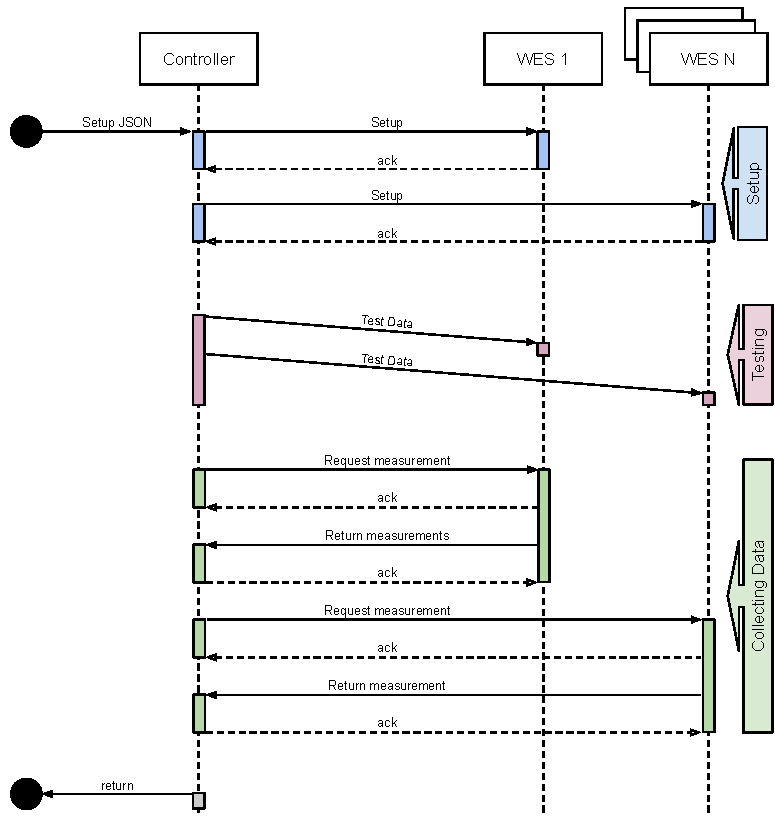
\includegraphics[scale=0.9]{figures/sequence_diagram_drive.pdf}
	\caption{Sequence Diagram of the Measurment}
	\label{fig:sequenceDiagram}
\end{figure}

\section{Wireshark measurements}

The Wireshark tool is suitable for recording traffic.
In order to record packets outside of a LAN, the WIFI card must be set to monitor mode.
In this mode, frames from an ad-hoc network can also be sniffed, as is the case with ESP-NOW.
In \cref{fig:wiresharkUC} it is clear to see that each unicast is followed by an acknolegement, as mentioned in the Chapter 3.

\begin{figure}[h]
	\centering
	\includegraphics[scale=0.5]{figures/wiresharkUC.pdf}
	\caption{Unicast Transmissions Recording from Wireshark}
	\label{fig:wiresharkUC}
\end{figure}

A look into the data frame \cref{fig:wiresharkUCTransmission} also shows the measured airtime of 696$\mu$s.
Adding the average backoff of a free channel (160$\mu$s) and the DIFS (50$\mu$s) gives 906$\mu$s.
In the calculation from \cref{tab:airtime_unicast_calc}, however, it was only 746$\mu$s.
\todo{TOLJA!\\yes.... actually why?}The difference of 120$\mu$s can be... 
Wireshark also recognises the category code of the Vendor Specific Action Frame that ESP-NOW uses.
The payload of 20 bytes assumed for unicast in the experiment is given here as 31 bytes,
presumably it has to do with the implementation of the action frame shown in \cref{fig:esp_now_vendor_format},
even though I can only figure out an offset of 10 bytes.\todo{is this personal note OK?}

\begin{figure}[h]
	\centering
	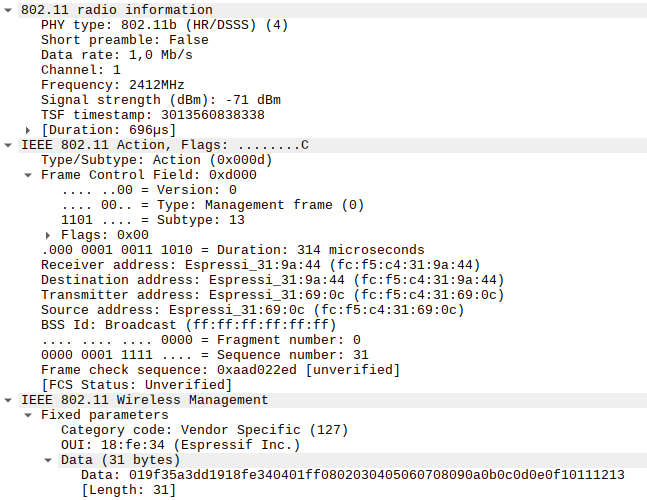
\includegraphics[scale=0.4]{figures/wiresharkUCFrame.png}
	\caption{Unicast Transmission Radio Information from Wireshark}
	\label{fig:wiresharkUCTransmission}
\end{figure}

\href{lst:callback}
A look at the 31 byte "payload" shows that ESP-NOW specific parts of wireshark have not been parsed correctly.
From the representation \cref{fig:esp-now_frame_format} and \cref{fig:esp-now_frame_format} it can be deduced:

that the first 4 bytes of the payload are still the random values and, according to Espressif, 
do not belong to the Vendor Specific Content.
These 4 bytes together with the following 1 byte (Element ID), 1 byte (length, interestingly specified as 25 Byte instead of 20),
Organisation Identifier (3 bytes), Type (1 byte) and Version (1 byte) make up the difference of 11 bytes to the actual payload.
\todo{This is barely readable}
The payload is filled with the flag ff \cref{lst:callback} followed by the sequence number, in this example 0.
The rest of the payload is filled with numbers, which are set to the value of the position in the payload.

\begin{figure}[h]
	\centering
	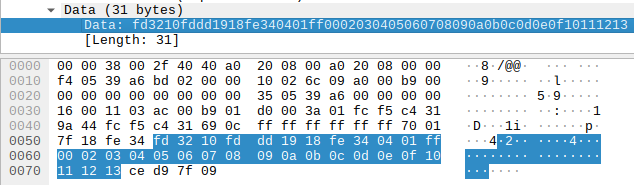
\includegraphics[scale=0.4]{figures/wiresharkPayload.png}
	\caption{Unicast Payload Analysis with Wireshark}
	\label{fig:wiresharkPayload}
\end{figure}

For completeness, here is a recording of the broadcast traffic.
The difference to the unicast traffic in \cref{fig:wiresharkUCTransmission} is,
that the destination address is bundled in a transmission of 160 bytes instead of being distributed in 8x20 byte packets.
As already mentioned, the acknoledgments are not possible with the broadcast.

\begin{figure}[h]
	\centering
	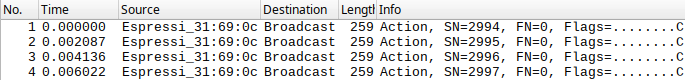
\includegraphics[scale=0.5]{figures/wiresharkBC.png}
	\caption{Unicast Payload Analysis with Wireshark}
	\label{fig:wiresharkBCTransmission}
\end{figure}

\section{Protocols under Study}

\subsection*{Slim Unicast vs Slim Broadcast}

In the design part it became clear that it is much more efficient 
to reach many individual WESs with one broadcast instead of many individual unicasts.
Tracking the transmissions with Wireshark also confirms this assumption \cref{fig:transmissionTime}.

\begin{figure}[h]
	\centering
	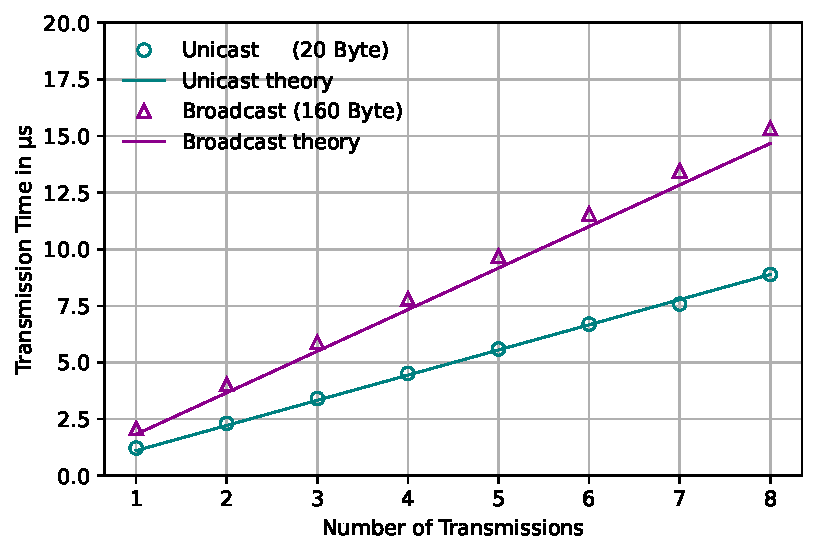
\includegraphics[scale=0.6]{../Plot2/Graphs/bc_uc_transmissiontime_wireshark.pdf}
	\caption{E.g. Transmission Time of Slim Unicast and Slim Broadcast}
	\label{fig:transmissionTime}
\end{figure}
\todo{Improve Graph. Transmissions is unclear}

The theoretical assumptions clearly correspond to the measured values,
Additional latencies due to processing in the microcontroller or at the antenna are therefore hardly significant.
When evaluating the graph, however, 
it should be noted that eight unicast transmissions have the same payload as a single broadcast transmission, by a factor of 4.
Therefore, a broadcast is clearly superior to a unicast in terms of latency, update frequency and synchronisation.

Slim Unicast can only make a difference through its reliability.
The channel in the experiment was free, so no retransmissions had to be sent, which would have delayed the transmission time even more.
When implementing slim unicast, it makes sense to do without synchronisation, because the buffering delay would be too long.
However, it is also difficult to estimate how many transmissions can be saved if only changed values trigger a transmission,
but it makes sense to simulate a stress test because critical errors become apparent precisely
when packets are lost and all values are changed.

It can be said that Slim Broadcast is the superior design due to the much lower part of overhead, 
because the data throughput is significantly higher.
The WESs can also be synchronised more easily because the transmissions reach many people at the same time.
The weak point, however, is reliability.

\subsection*{Rapid Repetition}
\todo{how to show 100\% success ratio?}

Success Ratio is a good metric to measure reliability, 
it is calculated from the number of successfully received packets and the total number of packets sent.
In a test setup of 7 distributed WESs, some placed close to the controller, some at a slightly greater distance,
this naturally varies greatly \cref{fig:sr_broadcast}.
The measurement was carried out in a flat distributed over different rooms.
Several WLANs are on the 2.4GHz band and lead to indifferences.
For the slim broadcast, 160Byte packets were distributed in a 600 sequence. the experiment was repeated 1000 times.

\begin{figure}[h]
	\centering
	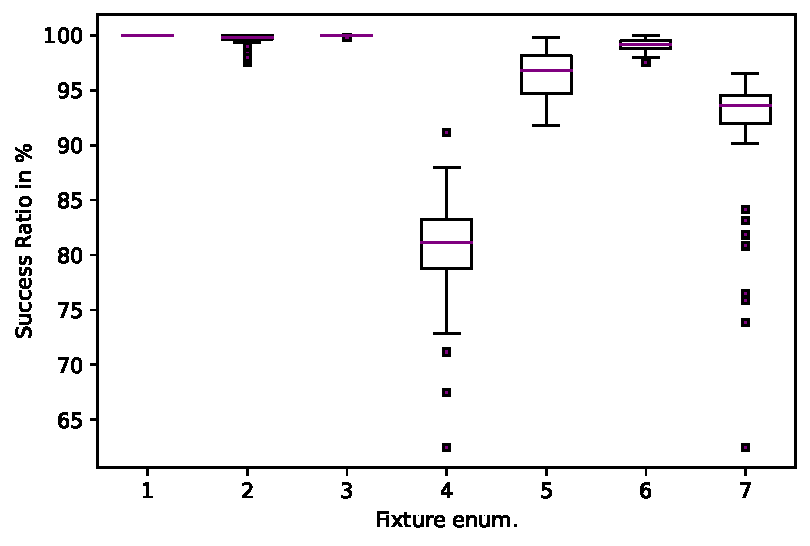
\includegraphics[scale=0.6]{../Plot2/Graphs/SR_per_fixture_broadcast.pdf}
	\caption{SR des Broadcasts aller 7 WESs}
	\label{fig:sr_broadcast}
\end{figure}

It shows that especially WESs 4 and WES 7 have poor reception.
The reception of other WESs is much better.
It should be said that with the Slim Unicast 100\% of the packets arrived and there was no loss of data.
One approach to improving reliability at the expense of latency was rapid repetitions.

With RR, it must be weighed up how many repetitions are sensible, 
because at some point the performance beyond reliability is impaired too much.
WES4 has the weakest reception and is supposed to represent a kind of worst-case scenario.
The measurement data of the same measurement as for \cref{fig:sr_broadcast} are used as a basis,
so that a comparability is given.
With RR=0, the unchanged SR is taken over, with RR=X, X transmissions are always linked in pairs to one with an or.

\begin{figure}[h]
	\centering
	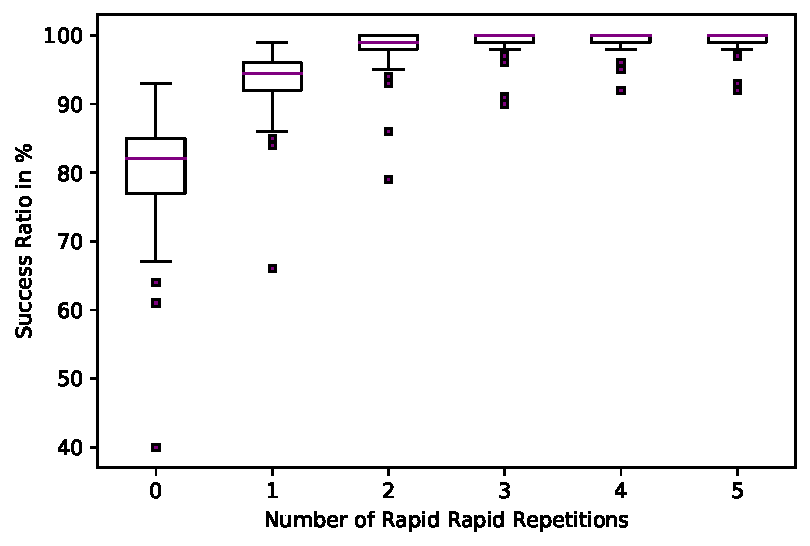
\includegraphics[scale=0.6]{../Plot2/Graphs/SR_of_node4_rr.pdf}
	\caption{SR of WES4 with altered RRs}
	\label{fig:sr_broadcast_wes4}
\end{figure}

It becomes clear that even a few repetitions lead to a significantly better SR.
But it also becomes clear that this is no longer improved as much after two repetitions.
However, a reliability of 100\% as with unicast is not necessarily achieved.
A look at the measurement data shows why \cref{fig:rrBitwise}.

\begin{figure}[h]
	\centering
	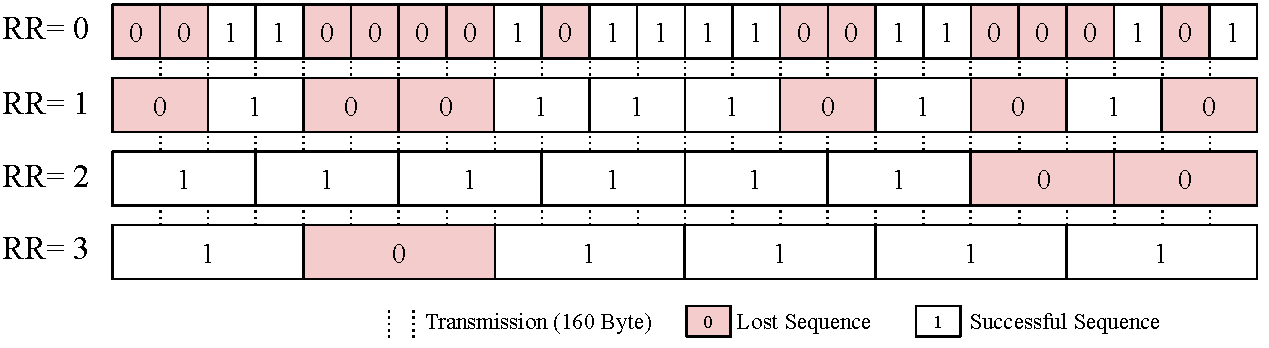
\includegraphics[scale=0.5]{figures/rrBitwise.pdf}
	\caption{Bitwise Example of RR (WES=4, SeqNr.=9-24, ExpNr.=1)}
	\label{fig:rrBitwise}
\end{figure}

The given excerpt is from an actual measurement of the WES4, 
the channel here is really very bad and there is massive packet loss.
When the repetitions are increased from RR=0 to RR=1, the loss of packets is slightly dampened.
However, it is noticeable that even with RR=3,
one sequence is still lost, despite the 4x costs of latency and throughput.
The problem is that faulty packets often come clustered 
and the repetitions still fall within the range of the bad channel.

\subsection*{Delayed Repetition}

To circumvent this circumstance, the sequences can be nested \cref{fig:badChannel},
this is only possible in combination with the Rapid Repetitions.
Subsequently swapping the sequence numbers makes it possible to make an evaluation on the same data.
WES4 is chosen again because the packet loss is greatest here.

\begin{figure}[h]
	\centering
	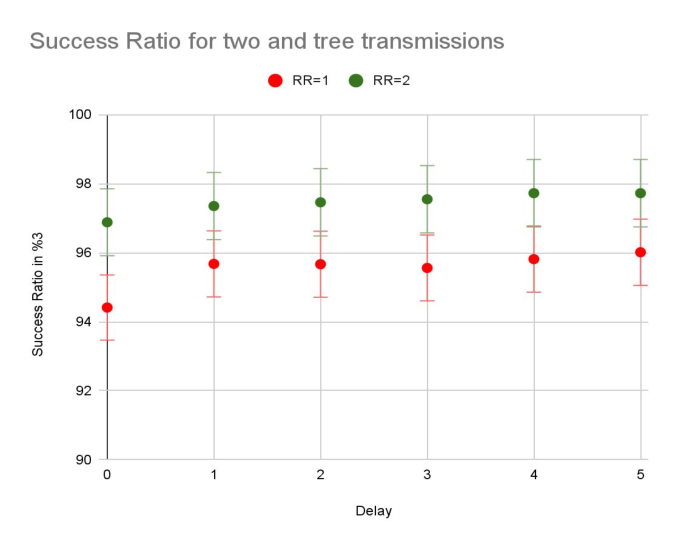
\includegraphics[scale=0.8]{figures/bufferingDelay.pdf}
	\caption{SR for Buffering Delay with/without RR for WES4}
	\label{fig:bufferingDelay}
\end{figure}
\todo{update Graphic!}

In \cref{fig:bufferingDelay} it is quite clear that the success ratio increases the longer the delay of the repetition.
However, the improvement converges quite quickly.
It can therefore be assumed that the success ratio is noticeably improved with a constant update frequency, 
at least with a buffering delay of 1, is the effect significant. \todo{How significant - after the plot is updated, give an exact example}
It also shows that the use of the buffering delay does not improve the success ratio so much 
that one less repetition could be sent.
In addition, the use of buffering delay has a cost in latency, as mentioned in FIGURE. \todo{link to graphic of buffering delay latency theory}.
It must therefore be weighed up whether the additional latency justifies the increased success ratio.

\subsection*{Impact of Groupsize}

\todo{optional}
When controlling lighting installations, the human eye does not notice so clearly 
if all lights are switched synchronously but with a delay.
However, it is clearly noticeable when a single light reacts with a delay.
With the BUffering Delay, synchronisation can be achieved, 
but what happens if a control signal does not arrive even despite RR and BD?
In the following, the Success Ratio is only considered successful if the control signals have arrived at all WESs.

\TODO{optional: SR Figure, different approaches with groupsize of 7, UC, BC, RR=1, RR=1+DR=1 RR=2, RR=2+DR+1, RR=3. RR=3+DR=1, RR=3+DR+2}

Evaluation \todo{optional: write evaluation}

\section{Results}
\TODO{Difference between Results and Discussion?}
\begin{itemize}
	\item Which method had the best results?
	\item Tabelle mit allen Protokollen auflisten 
\end{itemize}



\chapter{Conclusion \& Discussion}
\begin{itemize}
\item summarize again what your paper did, but now emphasize more the results, and comparisons
\item write conclusions that can be drawn from the results found and the discussion presented in the paper
\item future work (be very brief, explain what, but not much how, do not speculate about results or impact)
\item recommended length: one page.
\end{itemize}

Why not 5GHz -> to expensive.\\


\section*{Keep in Mind}
\begin{itemize}
\item metrics (SR, Latency, ...)
\item compare with art-net all the time
\item wireshark
\end{itemize}

% \include{Guidelines}

\cleardoublepage

\listofabbreviations
\clearpage

\listoffigures
\clearpage

\listoftables
\clearpage

\lstlistoflistings
\clearpage

\printbibliography

\end{document}
